\documentclass[11pt,oneside]{article}	%use"amsart"insteadof"article"forAMSLaTeXformat
\usepackage{geometry}		%Seegeometry.pdftolearnthelayoutoptions.Therearelots.
\geometry{letterpaper}		%...ora4paperora5paperor...
%\geometry{landscape}		%Activateforforrotatedpagegeometry
%\usepackage[parfill]{parskip}		%Activatetobeginparagraphswithanemptylineratherthananindent
\usepackage{graphicx}				%Usepdf,png,jpg,orepsßwithpdflatex;useepsinDVImode
								%TeXwillautomaticallyconverteps-->pdfinpdflatex		
\usepackage{amssymb}
\usepackage{amsmath}
\usepackage{amsthm}
\newtheorem{definition}{Definition}
\newtheorem{theorem}{Theorem}
\newtheorem{example}{Example}
\usepackage[colorlinks]{hyperref}

%----macros begin---------------------------------------------------------------
\usepackage{color}
\usepackage{amsthm}

\def\conv{\mbox{\textrm{conv}\,}}
\def\aff{\mbox{\textrm{aff}\,}}
\def\E{\mathbb{E}}
\def\R{\mathbb{R}}
\def\Z{\mathbb{Z}}
\def\tex{\TeX}
\def\latex{\LaTeX}
\def\v#1{{\bf #1}}
\def\p#1{{\bf #1}}
\def\T#1{{\bf #1}}

\def\vet#1{{\left(\begin{array}{cccccccccccccccccccc}#1\end{array}\right)}}
\def\mat#1{{\left(\begin{array}{cccccccccccccccccccc}#1\end{array}\right)}}

\def\lin{\mbox{\rm lin}\,}
\def\aff{\mbox{\rm aff}\,}
\def\pos{\mbox{\rm pos}\,}
\def\cone{\mbox{\rm cone}\,}
\def\conv{\mbox{\rm conv}\,}
\newcommand{\homog}[0]{\mbox{\rm homog}\,}
\newcommand{\relint}[0]{\mbox{\rm relint}\,}

%----macros end-----------------------------------------------------------------

\title{The basic \texttt{larcc} module
\footnote{This document is part of the \emph{Linear Algebraic Representation with CoChains} (LAR-CC) framework~\cite{cclar-proj:2013:00}. \today}
}
\author{The LARCC team}
%\date{}							%Activatetodisplayagivendateornodate

\begin{document}
\maketitle
\nonstopmode

\tableofcontents
\newpage


\section{Basic representations}

A few basic representation of topology are used in LARCC. They include some common sparse matrix representations: CSR (Compressed Sparse Row),  CSC (Compressed Sparse Column),   COO (Coordinate Representation), and BRC (Binary Row Compressed). 

\subsection{BRC (Binary Row Compressed)}

We denote as BRC (Binary Row Compressed) the standard input representation of our LARCC framework. A BRC representation is an array of arrays of integers, with no requirement of equal length for the component arrays. The BRC format is used to represent a (normally sparse) binary matrix. Each component array corresponds to a matrix row, and contains the indices of columns that store a 1 value. No storage is used for 0 values.

\paragraph{BRC format example}

Let $A = (a_{i,j} \in \{0,1\})$ be a binary matrix. The notation $\texttt{BRC}(A)$ is used for the corresponding data structure.
\[
A = \mat{
0,1,0,0,0,0,0,1,0,0\\
0,0,1,0,0,0,0,0,0,0\\
1,0,0,1,0,0,0,0,0,1\\
1,0,0,0,0,0,1,0,0,0\\
0,0,0,0,0,1,1,1,0,0\\
0,0,1,0,1,0,0,0,1,0\\
0,0,0,0,0,0,0,0,0,0\\
0,1,0,0,0,0,0,1,0,1\\
0,0,0,1,0,0,0,0,1,0\\
0,1,1,0,1,0,0,0,0,0\\
}
\qquad\mapsto\qquad \texttt{BRC}(A) =
\begin{minipage}[c]{5cm}
\begin{verbatim}
[[1,7],
 [2],
 [0,3,9],
 [0,6],
 [5,6,7],
 [2,4,8],
 [],
 [1,7,9],
 [3,8],
 [1,2,4]]
\end{verbatim}
\end{minipage}
\]


\subsection{Format conversions}

\paragraph{From triples to \texttt{scipy.sparse}}
The function \texttt{brc2Coo} transforms a \texttt{BRC} representation in a list of triples (\emph{row}, \emph{column}, 1) ordered by row.
%-------------------------------------------------------------------------------
@D Brc to Coo transformation
@{def brc2Coo(ListOfListOfInt):
	COOm = [[k,col,1] for k,row in enumerate(ListOfListOfInt)
			for col in row ]
	return COOm
@}
%-------------------------------------------------------------------------------

Two coordinate compressed sparse matrices \texttt{cooFV} and \texttt{cooEV} are created below, starting from the \texttt{BRC} representation \texttt{FV} and \texttt{EV} of the incidence of vertices on faces and edges, respectively, for a very simple plane triangulation.
%-------------------------------------------------------------------------------
@D Test example of Brc to Coo transformation
@{print "\n>>> brc2Coo"
V = [[0, 0], [1, 0], [2, 0], [0, 1], [1, 1], [2, 1]]
FV = [[0, 1, 3], [1, 2, 4], [1, 3, 4], [2, 4, 5]]
EV = [[0,1],[0,3],[1,2],[1,3],[1,4],[2,4],[2,5],[3,4],[4,5]]
cooFV = brc2Coo(FV)
cooEV = brc2Coo(EV)
assert cooFV == [[0,0,1],[0,1,1],[0,3,1],[1,1,1],[1,2,1],[1,4,1],[2,1,1],
[2,3,1], [2,4,1],[3,2,1],[3,4,1],[3,5,1]]
assert cooEV == [[0,0,1],[0,1,1],[1,0,1],[1,3,1],[2,1,1],[2,2,1],[3,1,1],
[3,3,1],[4,1,1],[4,4,1],[5,2,1],[5,4,1],[6,2,1],[6,5,1],[7,3,1],[7,4,1],
[8,4,1],[8,5,1]]
@}
%-------------------------------------------------------------------------------
\paragraph{Conversion to \texttt{csr} format}

Then we give the function \texttt{triples2mat} to make the transformation from the sparse matrix, given as a list of triples \emph{row,column,value} (non-zero elements), to the \texttt{scipy.sparse} format corresponding to the \texttt{shape} parameter, set by default to \texttt{"csr"}, that stands for \emph{Compressed Sparse Row}, the normal matrix format of the LARCC framework. 
%-------------------------------------------------------------------------------
@D From list of triples to scipy.sparse
@{def triples2mat(triples,shape="csr"):
	n = len(triples)
	data = arange(n)
	ij = arange(2*n).reshape(2,n)
	for k,item in enumerate(triples):
		ij[0][k],ij[1][k],data[k] = item
	return scipy.sparse.coo_matrix((data, ij)).asformat(shape)
@}
%-------------------------------------------------------------------------------
The conversion from triples to \texttt{csr} format is provided below.
%-------------------------------------------------------------------------------
@D Coo to Csr transformation
@{def coo2Csr(COOm):
	CSRm = triples2mat(COOm,"csr")
	return CSRm
@}
%-------------------------------------------------------------------------------
Two CSR sparse matrices \texttt{csrFV} and \texttt{csrEV} are generated (by \emph{scipy.sparse})  in the following example:
%-------------------------------------------------------------------------------
@D Test example of Coo to Csr transformation
@{csrFV = coo2Csr(cooFV)
csrEV = coo2Csr(cooEV)
print "\ncsr(FV) =\n", repr(csrFV)
print "\ncsr(EV) =\n", repr(csrEV)
@}
%-------------------------------------------------------------------------------
The \emph{scipy} printout of the last two lines above is the following:
%-------------------------------------------------------------------------------
{\small
\begin{verbatim}
csr(FV) = <4x6 sparse matrix of type '<type 'numpy.int64'>'
		   with 12 stored elements in Compressed Sparse Row format>
csr(EV) = <9x6 sparse matrix of type '<type 'numpy.int64'>'
		   with 18 stored elements in Compressed Sparse Row format>
\end{verbatim}}
%-------------------------------------------------------------------------------

\paragraph{Conversion from \texttt{BRC} to \texttt{CSR} format}
The transformation from BRC to CSR format is implemented slightly differently, according to the fact that the matrix dimension is either unknown (\texttt{shape=(0,0)}) or known.
%-------------------------------------------------------------------------------
@D Brc to Csr transformation
@{def csrCreate(BRCmatrix,lenV=0,shape=(0,0)):
	triples = brc2Coo(BRCmatrix)
	if shape == (0,0):
		CSRmatrix = coo2Csr(triples)
	else:
		CSRmatrix = scipy.sparse.csr_matrix(shape)
		for i,j,v in triples: CSRmatrix[i,j] = v
	return CSRmatrix
@}
%-------------------------------------------------------------------------------

\paragraph{Example}
The conversion to CSR format of the characteristic matrix \emph{faces-vertices} \texttt{FV} is given below for our simple example made by four triangle of a manifold 2D space, graphically shown in Figure~\ref{fig:2D-non-manifold}a. The LAR representation with CSR matrices does not make difference between manifolds and non-manifolds, conversely than most modern solid modelling representation schemes, as shown by removing from \texttt{FV} the third triangle, giving the model in Figure~\ref{fig:2D-non-manifold}b.
%-------------------------------------------------------------------------------
@D Test example of Brc to Csr transformation
@{print "\n>>> brc2Csr"
V = [[0, 0], [1, 0], [2, 0], [0, 1], [1, 1], [2, 1]]
FV = [[0, 1, 3], [1, 2, 4], [1, 3, 4], [2, 4, 5]]
EV = [[0,1],[0,3],[1,2],[1,3],[1,4],[2,4],[2,5],[3,4],[4,5]]
csrFV = csrCreate(FV)
csrEV = csrCreate(EV)
print "\ncsrCreate(FV) =\n", csrFV
VIEW(STRUCT(MKPOLS((V,FV))))
VIEW(STRUCT(MKPOLS((V,EV))))
@}
%-------------------------------------------------------------------------------

\begin{figure}[htbp] %  figure placement: here, top, bottom, or page
   \centering
   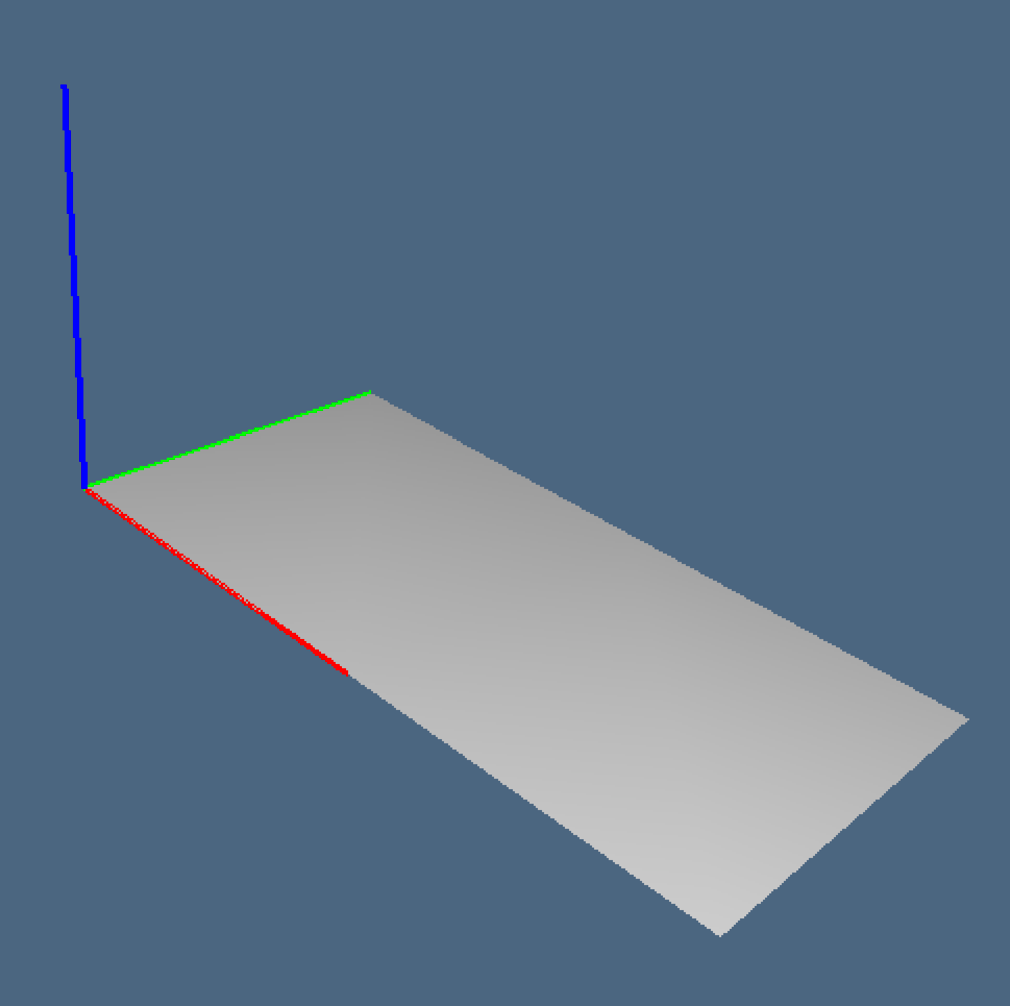
\includegraphics[height=0.25\linewidth,width=0.25\linewidth]{images/larcc1a} 
   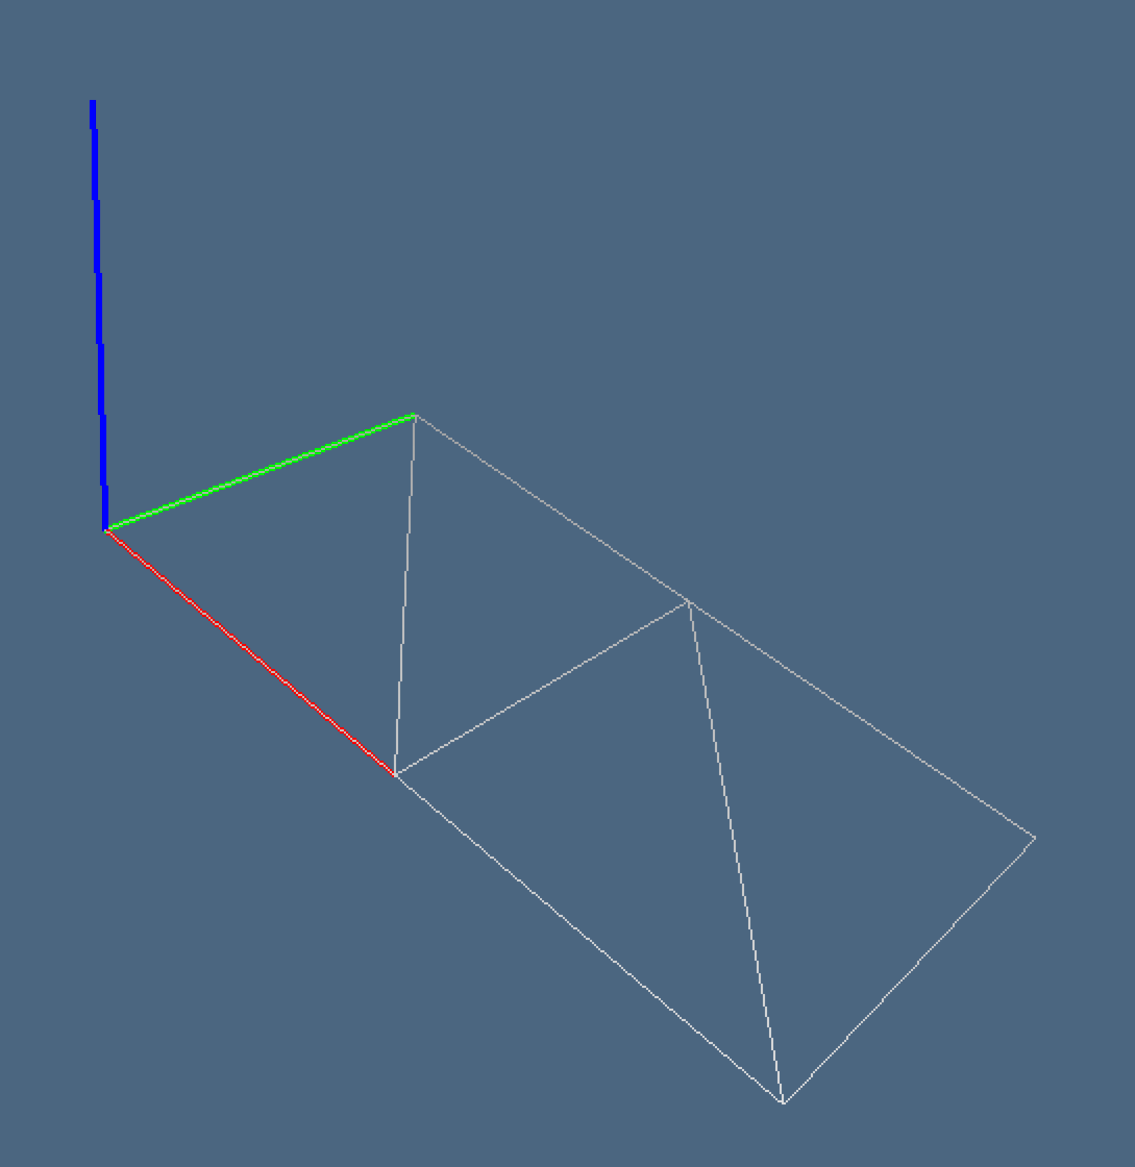
\includegraphics[height=0.25\linewidth,width=0.25\linewidth]{images/larcc1b} 
   \caption{(a) Simplicial 2-complex; (b) its 1-skeleton.}
   \label{fig:2D-non-manifold}
\end{figure}

\section{Matrix operations}

As we know, the LAR representation of topology is based on CSR representation of sparse binary (and integer) matrices. In this section we hence discuss the stack of matrix representations and operations implemented by this module.  The current python prototype makes reference to the scipy implementation of sparse matrices. Later implementations in different languages will necessarily make reference to different matrix packages.


\subsection{Basic operations}

Two utility functions allow to query the number of rows and columns of a CSR matrix, independently from the low-level implementation (that in the following is provided by \emph{scipy.sparse}).
%-------------------------------------------------------------------------------
@D Query Matrix shape
@{def csrGetNumberOfRows(CSRmatrix):
	Int = CSRmatrix.shape[0]
	return Int
	
def csrGetNumberOfColumns(CSRmatrix):
	Int = CSRmatrix.shape[1]
	return Int
@}
%-------------------------------------------------------------------------------
%-------------------------------------------------------------------------------
@D Test examples of Query Matrix shape
@{print "\n>>> csrGetNumberOfRows"
print "\ncsrGetNumberOfRows(csrFV) =", csrGetNumberOfRows(csrFV)
print "\ncsrGetNumberOfRows(csrEV) =", csrGetNumberOfRows(csrEV)
print "\n>>> csrGetNumberOfColumns"
print "\ncsrGetNumberOfColumns(csrFV) =", csrGetNumberOfColumns(csrFV)
print "\ncsrGetNumberOfColumns(csrEV) =", csrGetNumberOfColumns(csrEV)
@}
%-------------------------------------------------------------------------------

\paragraph{Sparse to dense matrix transformation}
The Scipy package provides the useful method \texttt{.todense()} in order to transform any sparse matrix format in the corresponding dense format. The function \texttt{csr2DenseMatrix} is given here for the sake of generality and portability.

%-------------------------------------------------------------------------------
@D Sparse to dense matrix transformation
@{def csr2DenseMatrix(CSRm):
	nrows = csrGetNumberOfRows(CSRm)
	ncolumns = csrGetNumberOfColumns(CSRm)
	ScipyMat = zeros((nrows,ncolumns),int)
	C = CSRm.tocoo()
	for triple in zip(C.row,C.col,C.data):
		ScipyMat[triple[0],triple[1]] = triple[2]
	return ScipyMat
@}
%-------------------------------------------------------------------------------
%-------------------------------------------------------------------------------
@D Test examples of Sparse to dense matrix transformation
@{print "\n>>> csr2DenseMatrix"
print "\nFV =\n", csr2DenseMatrix(csrFV)
print "\nEV =\n", csr2DenseMatrix(csrEV)
@}
%-------------------------------------------------------------------------------


\paragraph{Matrix product and transposition}

The following macro provides the IDE interface for the two main matrix operations required by LARCC, the binary product of compatible matrices and the unary transposition of matrices.

%-------------------------------------------------------------------------------
@D Matrix product and transposition
@{def matrixProduct(CSRm1,CSRm2):
	CSRm = CSRm1 * CSRm2
	return CSRm

def csrTranspose(CSRm):
	CSRm = CSRm.T
	return CSRm
@}
%-------------------------------------------------------------------------------


\subsection{Characteristic matrices}

We define as \emph{characteristic matrices} $M_k$ ($0\leq k\leq d$) the binary matrices having as rows the images of the characteristic functions of the $k$-cells $\alpha_k\subset V$ of a cellular complex with vertices $V$.
Remember that characteristic (or \emph{indicator}) function is 
\[
\mathbf{1}_A\colon V \to \{0, 1\}, \qquad 
\]
which for a given subset $A$ of $X$, has value 1 at points of $A$ and 0 at points of $V - A$.
 
\paragraph{Example: from \texttt{BRC} to \texttt{CSR} to \texttt{dense} matrix} 
Let us compute and show in dense form the characteristic matrices of 2- and 1-cells of the simple manifold given in Figure~\ref{fig:2D-non-manifold}.
By running the file \texttt{test/py/larcc/test08.py} the reader will get the two matrices shown in Example~\ref{ex:denseMat}
%-------------------------------------------------------------------------------
@o test/py/larcc/test08.py
@{import sys; sys.path.insert(0, 'lib/py/')
from larcc import *
@< Test example of Brc to Csr transformation @>
@< Test examples of Sparse to dense matrix transformation @>
@}
%-------------------------------------------------------------------------------
 
\begin{example}[Dense Characteristic matrices]\label{ex:denseMat}
Let us notice that the two matrices below have the some numbers of columns (indexed by vertices of the cell decomposition).
This very fact allows to multiply one matrix for the other transposed, and hence to compute the matrix form of linear operators between the spaces of cells of various dimensions.
\[
\texttt{FV} =
\begin{minipage}[c]{0.29\linewidth}
\begin{verbatim}
[[1 1 0 1 0 0]
 [0 1 1 0 1 0]
 [0 1 0 1 1 0]
 [0 0 1 0 1 1]]
\end{verbatim}
\end{minipage}
\qquad
\texttt{EV} =
\begin{minipage}[c]{0.29\linewidth}
\begin{verbatim}
[[1 1 0 0 0 0]
 [1 0 0 1 0 0]
 [0 1 1 0 0 0]
 [0 1 0 1 0 0]
 [0 1 0 0 1 0]
 [0 0 1 0 1 0]
 [0 0 1 0 0 1]
 [0 0 0 1 1 0]
 [0 0 0 0 1 1]]
\end{verbatim}
\end{minipage}
\]
\end{example}

\begin{example}[Operators from edges to faces and vice-versa]\label{ex:denseMat}
As a general rule for operators between two spaces of chains of different dimensions supported by the \emph{same} cellular complex, we use names made by two characters, whose first letter correspond to the target space, and whose second letter to the domain space. Hence \texttt{FE} must be read as the operator from edges to faces. Of course, since this use correspond to see the first letter as the space generated by rows, and the second letter as the space generated by columns. Notice that the element $(i,j)$ of such matrices stores the number of vertices shared between the (row-)cell $i$ and the (column-)cell $j$.
\[
\texttt{FE} = \texttt{FV}\ \texttt{EV}^\top = 
\begin{minipage}[c]{0.29\linewidth}
\begin{verbatim}
[[2 2 1 2 1 0 0 1 0]
 [1 0 2 1 2 2 1 1 1]
 [1 1 1 2 2 1 0 2 1]
 [0 0 1 0 1 2 2 1 2]]
\end{verbatim}
\end{minipage}
\qquad
\texttt{EF} = \texttt{EV}\ \texttt{FV}^\top = 
\begin{minipage}[c]{0.29\linewidth}
\begin{verbatim}
[[2 1 1 0]
 [2 0 1 0]
 [1 2 1 1]
 [2 1 2 0]
 [1 2 2 1]
 [0 2 1 2]
 [0 1 0 2]
 [1 1 2 1]
 [0 1 1 2]]
\end{verbatim}
\end{minipage}
\]
\end{example}

\begin{figure}[htbp] %  figure placement: here, top, bottom, or page
   \centering
   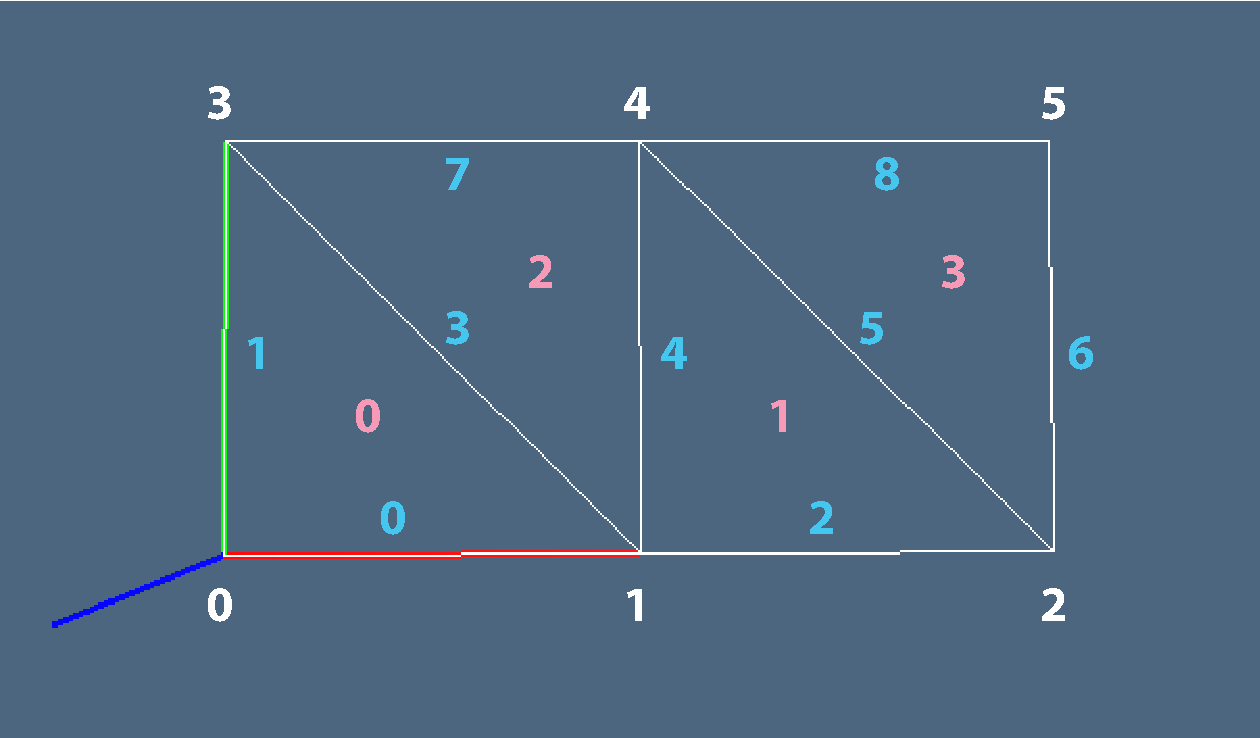
\includegraphics[width=0.6\linewidth]{images/2complex} 
   \caption{example caption}
   \label{fig:2complex}
\end{figure}

\paragraph{Matrix elements filtering}

Some filtering operations on matrix elements are needed in the implementation of various topological operators. Some of such filtering operations are given below.

%-------------------------------------------------------------------------------
@D Matrix filtering to produce the boundary matrix
@{def csrBoundaryFilter(CSRm, facetLengths):
	maxs = [max(CSRm[k].data) for k in range(CSRm.shape[0])]
	inputShape = CSRm.shape
	coo = CSRm.tocoo()
	for k in range(len(coo.data)):
		if coo.data[k]==maxs[coo.row[k]]: coo.data[k] = 1
		else: coo.data[k] = 0
	mtx = coo_matrix((coo.data, (coo.row, coo.col)), shape=inputShape)
	out = mtx.tocsr()
	return out
@}
%-------------------------------------------------------------------------------
%-------------------------------------------------------------------------------
@D Test example of Matrix filtering to produce the boundary matrix
@{print "\n>>> csrBoundaryFilter"
csrEF = matrixProduct(csrFV, csrTranspose(csrEV)).T
facetLengths = [csrCell.getnnz() for csrCell in csrEV]
CSRm = csrBoundaryFilter(csrEF, facetLengths).T
print "\ncsrMaxFilter(csrFE) =\n", csr2DenseMatrix(CSRm)
@}
%-------------------------------------------------------------------------------
%-------------------------------------------------------------------------------
@D Matrix filtering via a generic predicate
@{def csrPredFilter(CSRm, pred):
	# can be done in parallel (by rows)
	coo = CSRm.tocoo()
	triples = [[row,col,val] for row,col,val 
				in zip(coo.row,coo.col,coo.data) if pred(val)]
	i, j, data = TRANS(triples)
	CSRm = scipy.sparse.coo_matrix((data,(i,j)),CSRm.shape).tocsr()
	return CSRm
@}
%-------------------------------------------------------------------------------
%-------------------------------------------------------------------------------
@D Test example of Matrix filtering via a generic predicate
@{print "\n>>> csrPredFilter"
CSRm = csrPredFilter(matrixProduct(csrFV, csrTranspose(csrEV)).T, GE(2)).T
print "\nccsrPredFilter(csrFE) =\n", csr2DenseMatrix(CSRm)
@}
%-------------------------------------------------------------------------------


\subsection{Computation of lower-dimensional skeletons}

In most cases, in particular when the cellular complex is made by convex cells, the only cells of maximal dimension must be entered to gain a complete knowledge of the whole complex.
Here we show how to compute the $(d-1)$-skeleton of a complex starting from its $d$-dimensional skeleton.

\paragraph{Extraction of facets of a cell complex} 

The following \texttt{larFacets} function returns the LAR model \texttt{V,cellFacets} starting from the input \texttt{model} parameter. Two optional parameters define the (intrinsic) dimension of the input cells, with default value equal to three, and the eventual presence of a \texttt{emptyCellNumber} of empty cells. Their number default to zero when the complex is closed, for example in the case it provides the $d$-boundary of a $(d+1)$-complex. If empty cells are present, their subset must be located at the end of the \texttt{cell} list.

%-------------------------------------------------------------------------------
@D Extraction of facets of a cell complex
@{def setup(model,dim):
	V, cells = model
	csr = csrCreate(cells)
	csrAdjSquareMat = larCellAdjacencies(csr)
	csrAdjSquareMat = csrPredFilter(csrAdjSquareMat, GE(dim)) # ? HOWTODO ?
	return V,cells,csr,csrAdjSquareMat

def larFacets(model, dim=3, emptyCellNumber=0):
	""" Estraction of (d-1)-cellFacets from "model" := (V,d-cells)
		Return (V, (d-1)-cellFacets)
		"""
	V,cells,csr,csrAdjSquareMat = setup(model,dim)
	solidCellNumber = len(cells) - emptyCellNumber
	cellFacets = []
	# for each input cell i
	for i in range(len(cells)):
		adjCells = csrAdjSquareMat[i].tocoo()
		cell1 = csr[i].tocoo().col
		pairs = zip(adjCells.col,adjCells.data)
		for j,v in pairs:
			if (i<j) and (i<solidCellNumber):
				cell2 = csr[j].tocoo().col
				cell = list(set(cell1).intersection(cell2))
				cellFacets.append(sorted(cell))
	# sort and remove duplicates
	cellFacets = sorted(AA(list)(set(AA(tuple)(cellFacets))))
	return V,cellFacets
@}
%-------------------------------------------------------------------------------



%-------------------------------------------------------------------------------
@D Computation of cell adjacencies
@{def larCellAdjacencies(CSRm):
	CSRm = matrixProduct(CSRm,csrTranspose(CSRm))
	return CSRm
@}
%-------------------------------------------------------------------------------

\paragraph{Examples}
Two simple complexes are defined below by providing the pair \texttt{V,FV}.
In both cases the \texttt{EV} relation is computed via the \texttt{larFacets} function.
%-------------------------------------------------------------------------------
@D Test examples of Extraction of facets of a cell complex
@{""" A first (simplicial) example """
V = [[0.,0.],[3.,0.],[0.,3.],[3.,3.],[1.,2.],[2.,2.],[1.,1.],[2.,1.]]
FV = [[0,1,3],[1,2,4],[2,4,5],[3,4,6],[4,6,7],[5,7,8], # full
	[1,3,4],[4,5,7], # empty
	[0,1,2],[6,7,8],[0,3,6],[2,5,8]] # exterior		
_,EV = larFacets((V,FV),dim=2)
print "\nEV =",EV
VIEW(EXPLODE(1.5,1.5,1.5)(MKPOLS((V,EV))))

""" Another (cuboidal) example """
FV = [[0,1,6,7],[0,2,4,6],[4,5,6,7],[1,3,5,7],[2,3,4,5],[0,1,2,3]]
_,EV = larFacets((V,FV),dim=2)
print "\nEV =",EV
VV = AA(LIST)(range(len(V)))
VIEW(EXPLODE(1.5,1.5,1.5)(MKPOLS((V,EV))))
@}
%-------------------------------------------------------------------------------

\paragraph{Visualization of cell numbers}
The adjacentcy matrices between 2-cells and 1-cells are printed here. Finally, the complex is displayed by numbering with different colours and sizes (depending on the rank) the complex cells.
%-------------------------------------------------------------------------------
@D Test examples of Computation of cell adjacencies
@{
print "\n>>> larCellAdjacencies"
adj_2_cells = larCellAdjacencies(csrCreate(FV))
print "\nadj_2_cells =\n", csr2DenseMatrix(adj_2_cells)
adj_1_cells = larCellAdjacencies(csrCreate(EV))
print "\nadj_1_cells =\n", csr2DenseMatrix(adj_1_cells)

submodel = mkSignedEdges((V,EV))
VIEW(submodel)
VIEW(larModelNumbering(scalx=1,scaly=1,scalz=1)(V,[VV,EV,FV],submodel,2))
@}
%-------------------------------------------------------------------------------


\section{Topological operations}

In this section we provide the matrix representation of operators to compute the more important and useful topological operations on cellular complexes, and/or the indexed relations they return. We start the section by giving a graphical tool used to test the developed software, concerning the graphical writing of the full set of indices of the cells of every dimension in a 3D cuboidal complex.  

\subsection{Visualization of cellular complexes}

It is often necessary to have a visual picture of the generated structures and computations.
This section provides some quite versatile visualisation tools of both the cells and/or their integer indices.

\paragraph{Visualization of cell indices}
As already outlined, the \texttt{modelIndexing} function return the \emph{hpc} value assembling both the 1-skeletons of the cells of every dimensions, and the graphical output of their indices, located on the centroid of each cell, and displayed using colors and sizes depending on the \emph{rank} of the cell.

%-------------------------------------------------------------------------------
@D Visualization of cell indices
@{""" Visualization of cell indices """
from sysml import *
def modelIndexing(shape):
	V, bases = larCuboids(shape,True)
	# bases = [[cell for cell in cellComplex if len(cell)==2**k] for k in range(4)]
	color = [ORANGE,CYAN,GREEN,WHITE]
	nums = AA(range)(AA(len)(bases))
	hpcs = []
	for k in range(4):
		hpcs += [SKEL_1(STRUCT(MKPOLS((V,bases[k]))))]
		hpcs += [cellNumbering((V,bases[k]),hpcs[2*k])(nums[k],color[k],0.3+0.2*k)]
	return STRUCT(hpcs)
@}
%-------------------------------------------------------------------------------


%-------------------------------------------------------------------------------
@D Visualization of cell indices
@{""" Numbered visualization of a LAR model """
def larModelNumbering(scalx=1,scaly=1,scalz=1):
	def  larModelNumbering0(V,bases,submodel,numberScaling=1):
		color = [ORANGE,CYAN,GREEN,WHITE]
		nums = AA(range)(AA(len)(bases))
		hpcs = [submodel]
		for k in range(len(bases)):
			hpcs += [cellNumbering((V,bases[k]),submodel)
						(nums[k],color[k],(0.5+0.1*k)*numberScaling)]
		return STRUCT(hpcs)
		#return EXPLODE(scalx,scaly,scalz)(hpcs)
	return larModelNumbering0
@}
%-------------------------------------------------------------------------------



\paragraph{Drawing of oriented edges}
The following function return the \texttt{hpc} of the drawing with arrows of the oriented 1-cells of a 2D cellular complex. Of course, each edge orientation is from second to first vertex, independently from the vertex indices. Therefore, the edge orientation can be reversed by swapping the vertex indices in the 1-cell definition. 
%-------------------------------------------------------------------------------
@D Drawing of oriented edges
@{""" Drawing of oriented edges (2D) """
def mkSignedEdges (model,scalingFactor=1):
	V,EV = model
	assert len(V[0])==2
	hpcs = []
	times = C(SCALARVECTPROD)
	frac = 0.06*scalingFactor
	for e0,e1 in EV:
		v0,v1 = V[e0], V[e1]
		vx,vy = DIFF([ v1, v0 ])
		nx,ny = [-vy, vx]
		v2 = SUM([ v0, times(0.66)([vx,vy]) ])
		v3 = SUM([ v0, times(0.6-frac)([vx,vy]), times(frac)([nx,ny]) ])
		v4 = SUM([ v0, times(0.6-frac)([vx,vy]), times(-frac)([nx,ny]) ])
		verts,cells = [v0,v1,v2,v3,v4],[[1,2],[3,4],[3,5]]
		hpcs += [MKPOL([verts,cells,None])]
	hpc = STRUCT(hpcs)
	return hpc
@}
%-------------------------------------------------------------------------------

\paragraph{Example of oriented edge drawing}
An example of drawing of oriented edges is given in \texttt{test/py/larcc/test11.py} file, and in Figure~\ref{numberedcomplex}, showing both the numbering of the cells and the arrows indicating the edge orientation is illustrated in Figure~\ref{numberedcomplex}, where also the oriented boundary is shown.

\begin{figure}[htbp] %  figure placement: here, top, bottom, or page
   \centering
   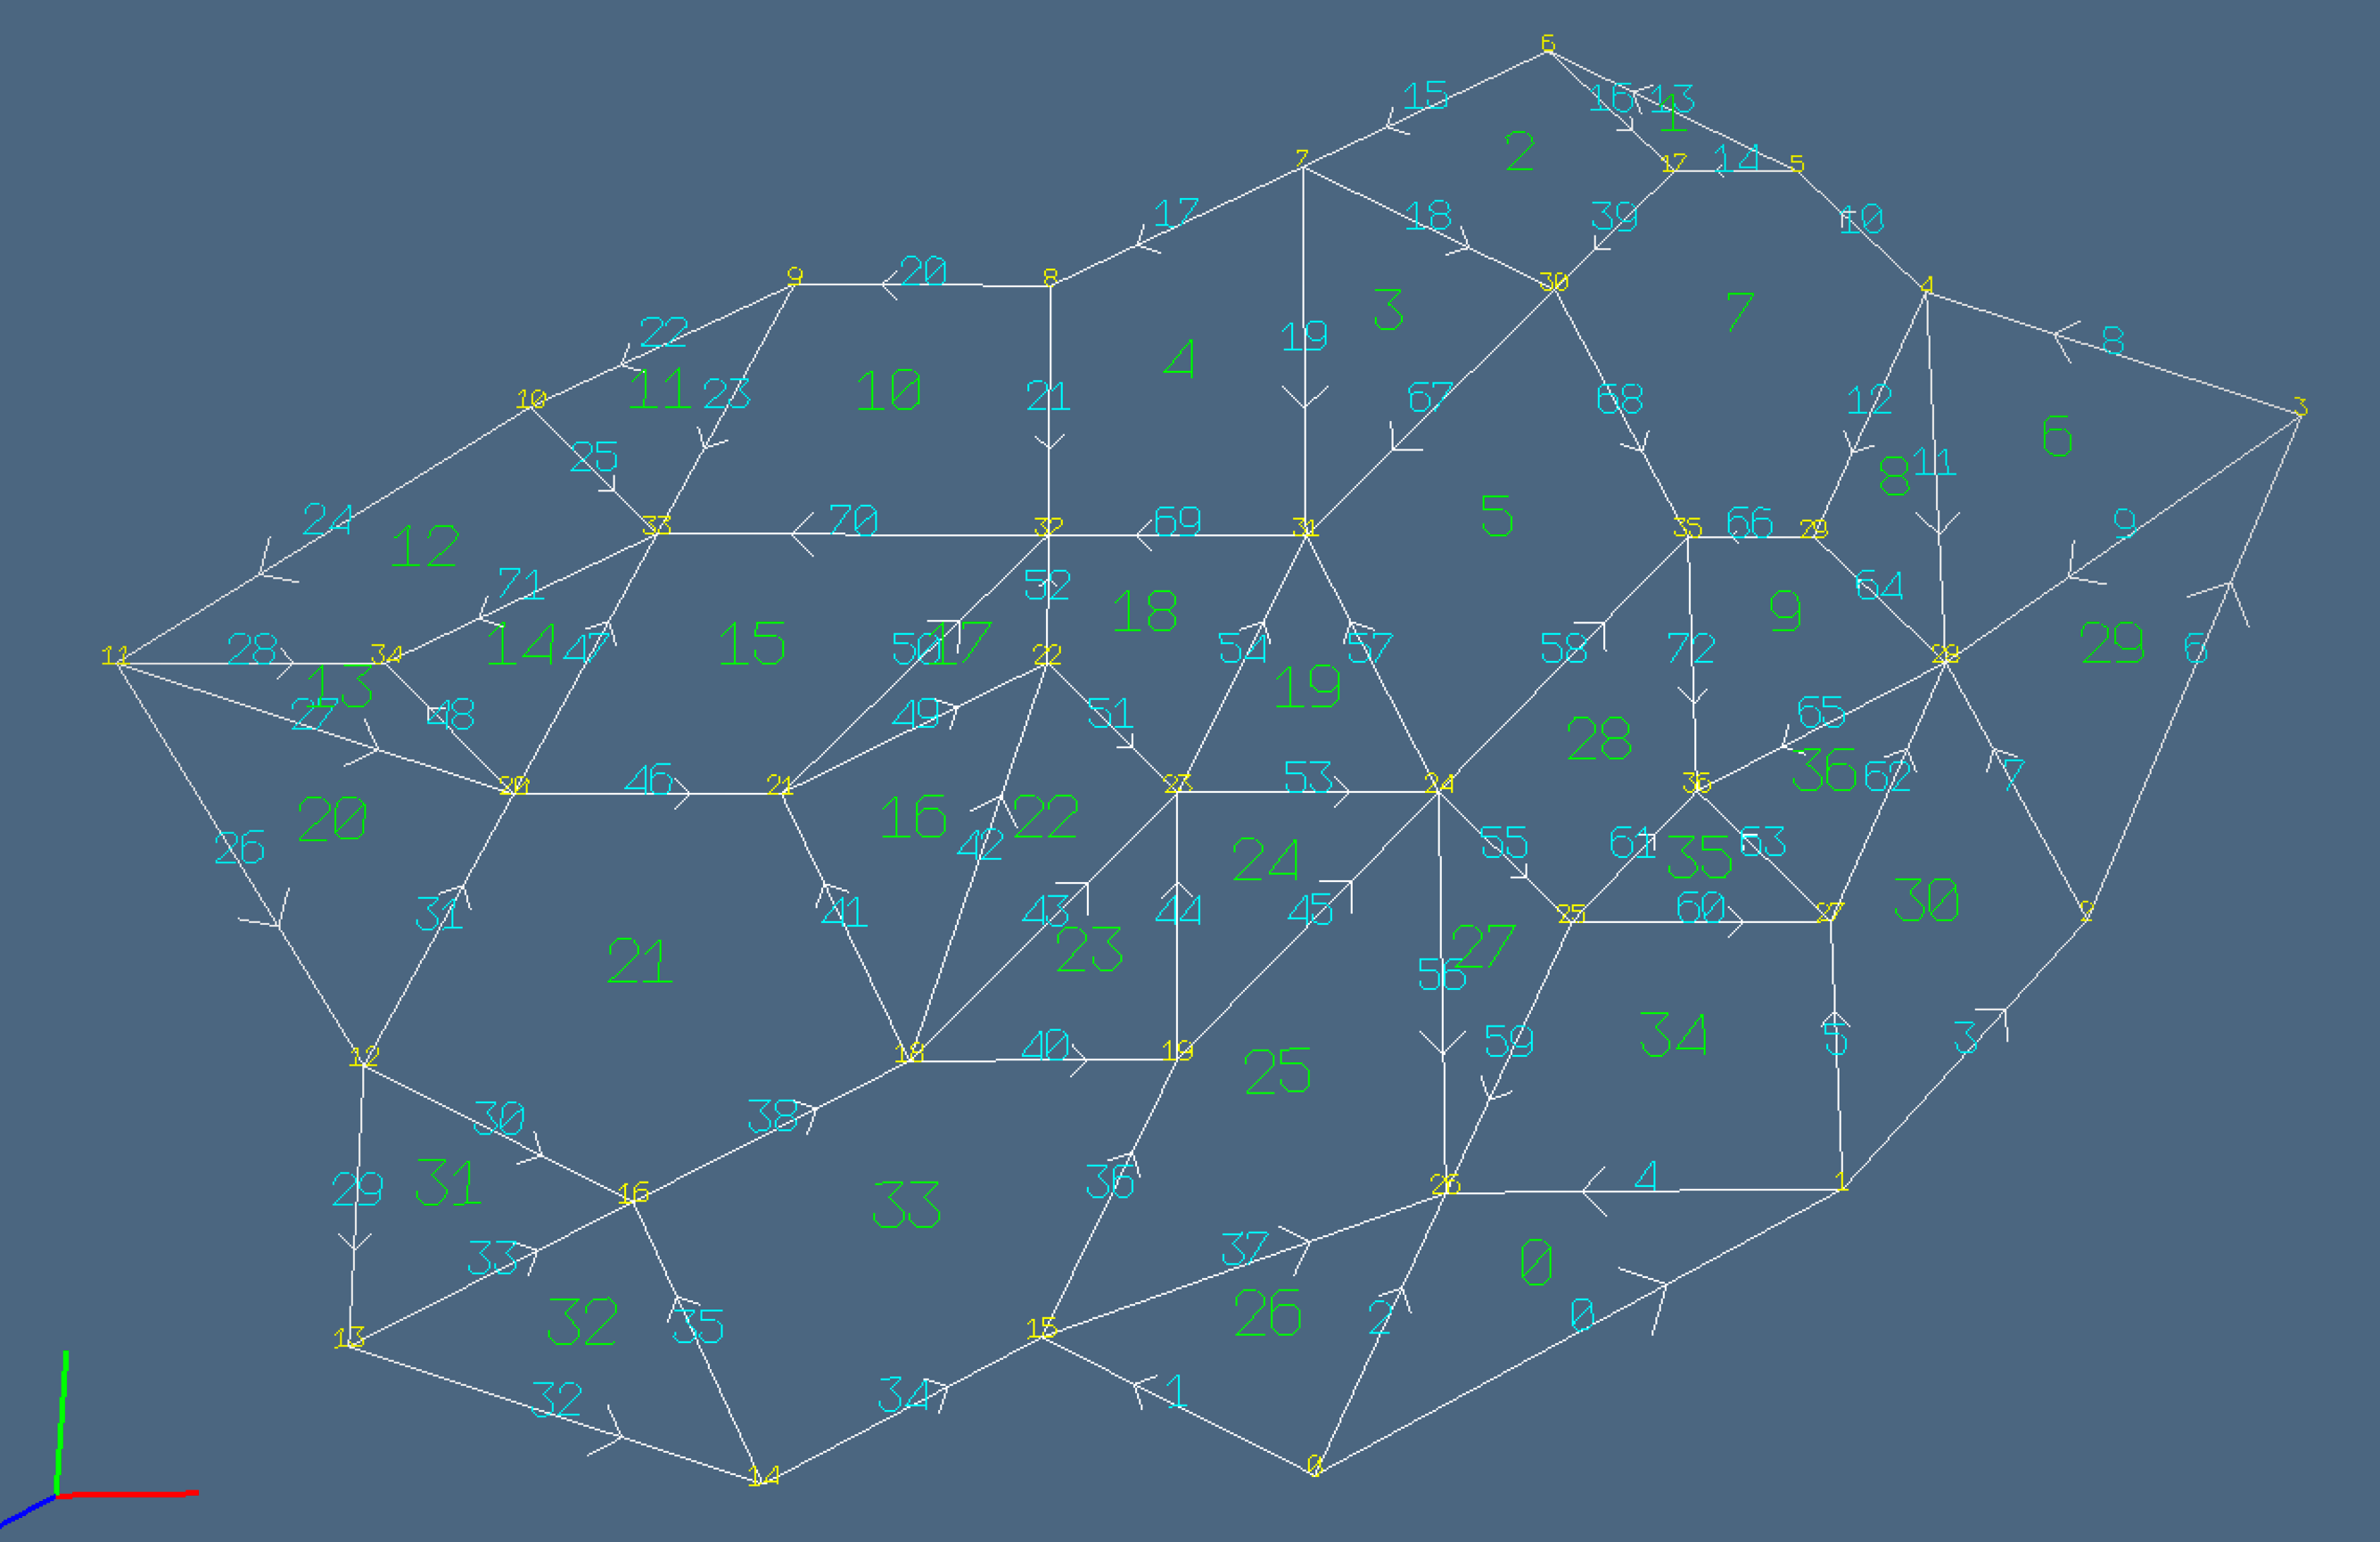
\includegraphics[width=0.9\linewidth]{images/numberedcomplex} 
   
   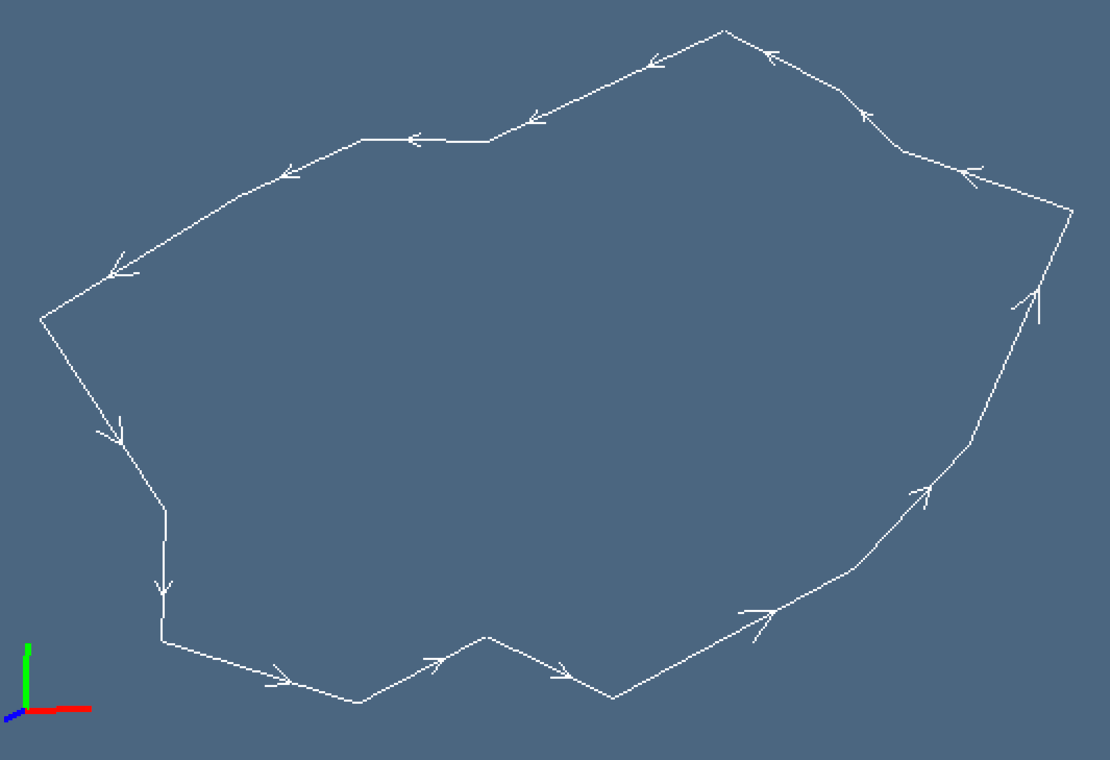
\includegraphics[width=0.9\linewidth]{images/numberedcomplex1} 
   \caption{Example of numbered polytopal complex, including edge orientations, and its oriented boundary.}
   \label{numberedcomplex}
\end{figure}

%-------------------------------------------------------------------------------
@O test/py/larcc/test11.py
@{""" Example of oriented edge drawing """
import sys;sys.path.insert(0, 'lib/py/')
from larcc import *

V = [[9,0],[13,2],[15,4],[17,8],[14,9],[13,10],[11,11],[9,10],[7,9],[5,9],[3,
8],[0,6],[2,3],[2,1],[5,0],[7,1],[4,2],[12,10],[6,3],[8,3],[3,5],[5,5],[7,6],
[8,5],[10,5],[11,4],[10,2],[13,4],[14,6],[13,7],[11,9],[9,7],[7,7],[4,7],[2,
6],[12,7],[12,5]]

FV = [[0,1,26],[5,6,17],[6,7,17,30],[7,30,31],[7,8,31,32],[24,30,31,35],[3,4,
28],[4,5,17,29,30,35],[4,28,29],[28,29,35,36],[8,9,32,33],[9,10,33],[11,10,
33,34],[11,20,34],[20,33,34],[20,21,32,33],[18,21,22],[21,22,32],[22,23,31,
32],[23,24,31],[11,12,20],[12,16,18,20,21],[18,22,23],[18,19,23],[19,23,24],
[15,19,24,26],[0,15,26],[24,25,26],[24,25,35,36],[2,3,28],[1,2,27,28],[12,13,
16],[13,14,16],[14,15,16,18,19],[1,25,26,27],[25,27,36],[36,27,28]]

VIEW(EXPLODE(1.2,1.2,1)(MKPOLS((V,FV))))
VV = AA(LIST)(range(len(V)))
_,EV = larFacets((V,FV+[range(16)]),dim=2,emptyCellNumber=1)

submodel = mkSignedEdges((V,EV))
VIEW(submodel)
VIEW(larModelNumbering(scalx=1,scaly=1,scalz=1)(V,[VV,EV,FV],submodel,2))

orientedBoundary = signedCellularBoundaryCells(V,[VV,EV,FV])
cells = [EV[e] if sign==1 else REVERSE(EV[e]) for (sign,e) in zip(*orientedBoundary)]
submodel = mkSignedEdges((V,cells))
VIEW(submodel)
@}
%-------------------------------------------------------------------------------


\subsection{Incidence and adjacency operators}

Let us start by computing the more interesting subset of the binary relationships between the 4 decompositive and/or boundary entities of 3D cellular models.  Therefore, in this case we denote with \texttt{C}, \texttt{F}, \texttt{E}, and \texttt{V}, the 3-cells and their faces, edges and vertices, respectively.
The input is the full-fledged LAR representation provided by 
\begin{align}
\texttt{CV} := \texttt{CSR}(M_3) \\
\texttt{FV} := \texttt{CSR}(M_2) \\
\texttt{EV} := \texttt{CSR}(M_1) \\
\texttt{VV} := \texttt{CSR}(M_0) 
\end{align}

Of course, $\texttt{CSR}(M_0)$ coincides with the identity matrix of dimension $|V|$ and can by excluded by further considerations.
Some binary incidence and adjacency relations we are going to compute are:
\begin{align}
\texttt{CF} := \texttt{CV} \times \texttt{FV}^t = \texttt{CSR}(M_3)\times\texttt{CSR}(M_2)^t \\
\texttt{CE} := \texttt{CV} \times \texttt{EV}^t = \texttt{CSR}(M_3)\times\texttt{CSR}(M_1)^t \\
\texttt{FE} := \texttt{FV} \times \texttt{EV}^t = \texttt{CSR}(M_2)\times\texttt{CSR}(M_1)^t 
\end{align}

The other possible operators follow from a similer computational pattern.

\paragraph{The programming pattern for incidence computation}

A high-level function \texttt{larIncidence} useful to compute the LAR representation of the incidence matrix (operator) and the incidence relations is given in the script below.

%-------------------------------------------------------------------------------
@D Some incidence operators
@{""" Some incidence operators """
def larIncidence(cells,facets):
	csrCellFacet = csrCellFaceIncidence(cells,facets)
	cooCellFacet = csrCellFacet.tocoo()
	larCellFacet = [[] for cell in range(len(cells))]
	for i,j,val in zip(cooCellFacet.row,cooCellFacet.col,cooCellFacet.data):
		if val == 1: larCellFacet[i] += [j]
	return larCellFacet

@< Cell-Face incidence operator @>
@< Cell-Edge incidence operator @>
@< Face-Edge incidence operator @>
@}
%-------------------------------------------------------------------------------


\paragraph{Cell-Face incidence}
The \texttt{csrCellFaceIncidence} and \texttt{larCellFace} functions are given below, and exported to the \texttt{larcc} module.
%-------------------------------------------------------------------------------
@D Cell-Face incidence operator
@{""" Cell-Face incidence operator """
def csrCellFaceIncidence(CV,FV):
	return boundary(FV,CV)

def larCellFace(CV,FV):
	return larIncidence(CV,FV)
@}
%-------------------------------------------------------------------------------

\paragraph{Cell-Edge incidence}
Analogously, the \texttt{csrCellEdgeIncidence} and \texttt{larCellFace} functions are given in the following script.

%-------------------------------------------------------------------------------
@D Cell-Edge incidence operator
@{""" Cell-Edge incidence operator """
def csrCellEdgeIncidence(CV,EV):
	 return boundary(EV,CV)

def larCellEdge(CV,EV):
	return larIncidence(CV,EV)
@}
%-------------------------------------------------------------------------------

\paragraph{Face-Edge incidence}
Finally, the \texttt{csrCellEdgeIncidence} and \texttt{larCellFace} functions are provided below.

%-------------------------------------------------------------------------------
@D Face-Edge incidence operator
@{""" Face-Edge incidence operator """
def csrFaceEdgeIncidence(FV,EV):
	return boundary(EV,FV)

def larFaceEdge(FV,EV):
	return larIncidence(FV,EV)
@}
%-------------------------------------------------------------------------------


\paragraph{Example}
The example below concerns a 3D cuboidal grid, by computing a full LAR stack of bases
\texttt{CV, FV, EV, VV}, showing its fully numbered 3D model, and finally by computing
some more useful binary relationships (\texttt{CF, CE, FE}), needed for example to compute the signed matrices of boundary operators.

%-------------------------------------------------------------------------------
@O test/py/larcc/test10.py
@{""" A mesh model and various incidence operators """
import sys; sys.path.insert(0, 'lib/py/')
from larcc import *
from largrid import *

shape = [2,2,2]
V,(VV,EV,FV,CV) = larCuboids(shape,True)
VIEW(modelIndexing(shape))

CF = larCellFace(CV,FV)
CE = larCellFace(CV,EV)
FE = larCellFace(FV,EV)
@}
%-------------------------------------------------------------------------------

\subsubsection{Incidence chain}

Let denote with \texttt{CF}, \texttt{FE}, \texttt{EV} the three consecutive incidence relations between $k$-cells and $(k-1)$-cells ($3\leq k\leq 0$) in a 3-complex. In the general multidimensional case, let us call \texttt{CF}$_d$  the generic \emph{binary} incidence operator, between $d$-cells and $(d-1)$-facets, as:
\[
\texttt{CF}_d = M_{d-1} M_d^t, 
\]
with
\[
\texttt{CF}_d := \{a_{ij}\}, \qquad a_{ij} = 
\left\{
\begin{array}{cl}
1 & \mbox{if\ } M_{d-1}(i) M_d(j) = |f_j|  \\
0 & \mbox{otherwise}  \\  
\end{array}
\right.
\]

\paragraph{Incidence chain computation}
The function \texttt{incidenceChain}, given below, returns the full stack of \texttt{BRC} incidence matrices of a LAR representation for a cellular complex, starting from its list of bases, i.e.~from \texttt{[VV,EV,FV,CV,...]}. Notice that the function returns the inverse sequence 
\texttt{[EV,FE,CF,...]}, i.e., \texttt{CF}$_k$ ($1\leq k\leq d$).

%-------------------------------------------------------------------------------
@D Incidence chain computation
@{""" Incidence chain computation """
def incidenceChain(bases):
	print "\n len(bases) = ",len(bases),"\n"
	pairsOfBases = zip(bases[1:],bases[:-1])
	relations = [larIncidence(cells,facets) 
					for cells,facets in pairsOfBases]
	return REVERSE(relations)
@}
%-------------------------------------------------------------------------------

%-------------------------------------------------------------------------------
@O test/py/larcc/test13.py
@{""" Example of incidence chain computation """
import sys; sys.path.insert(0, 'lib/py/')
from larcc import *
from largrid import *

shape = (1,1,2) 
print "\n\nFor a better example provide a greater shape!"
V,bases = larCuboids(shape,True)

VV,EV,FV,CV = bases
incidence = incidenceChain([VV,EV,FV,CV])
relations = ["CF","FE","EV"]
for k in range(3):
	print "\n\n incidence", relations[k], "=\n", incidence[k],
print "\n\n"

submodel = SKEL_1(STRUCT(MKPOLS((V,EV))))
VIEW(larModelNumbering(scalx=1,scaly=1,scalz=1)(V,[VV,EV,FV,CV],submodel,1))
@}
%-------------------------------------------------------------------------------


\paragraph{Example of incidence chain computation}
When running the \texttt{test/py/larcc/test13.py} file one obtains the following printout. 
Notice that 
it provides the links between $d$-cell numerations and the numerations of their faces.
See Figure~\ref{incidenceChain} for this purpose.

\begin{figure}[htbp] %  figure placement: here, top, bottom, or page
   \centering
   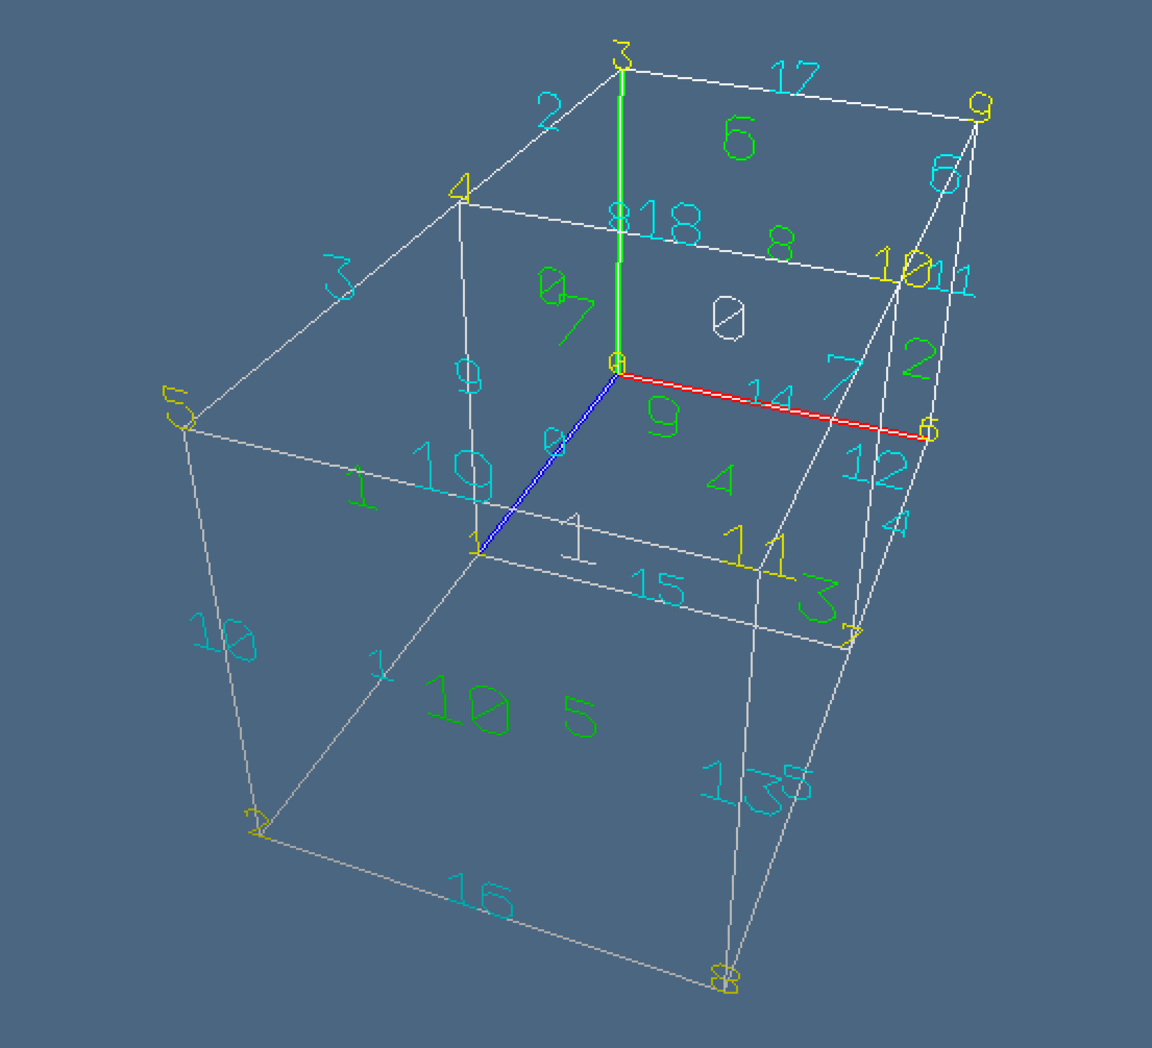
\includegraphics[width=0.5\linewidth]{images/incidenceChain} 
   \caption{Che stack of incidence relations gives the common links between cell numerations.}
   \label{incidenceChain}
\end{figure}


%-------------------------------------------------------------------------------
@D Incidence chain for a 3D cuboidal complex
@{incidence CF = [[0,2,4,6,8,9],[1,3,5,7,9,10]]

incidence FE = [[0,2,8,9],[1,3,9,10],[4,6,11,12],[5,7,12,13],[0,4,14,15],
[1,5,15,16],[2,6,17,18],[3,7,18,19],[8,11,14,17],[9,12,15,18],[10,13,16,19]]

incidence EV = [[0,1],[1,2],[3,4],[4,5],[6,7],[7,8],[9,10],[10,11],[0,3],
[1,4],[2,5],[6,9],[7,10],[8,11],[0,6],[1,7],[2,8],[3,9],[4,10],[5,11]]
@}
%-------------------------------------------------------------------------------



\subsection{Boundary and coboundary operators}

When computing the matrices of boundary and coboundary operators it may be useful to distinguish between simplicial complexes and general polytopal complexes, including  cuboidal ones. In the first cases all skeletons, and hence the other topological operators, may be computed using only combinatorial methods. In the second case some reference to their geometric embedding must be done, at least to compute the \emph{oriented} boundary and coboundary. Therefore we separate the two cases in the following sections.


\subsubsection{Non-oriented operators}

The \texttt{boundary} function below takes as parameters the \texttt{BRC} representations of $d$-cells and $(d-1)$-facets, and returns the \texttt{CSR} matrix of the boundary operator. Let us notice that such operator uses a mod 2 algebra, since it takes elements within the field $\Z_2=\{0,1\}$.

%-------------------------------------------------------------------------------
@D Test examples of From cells and facets to boundary operator
@{V = [[0.0,0.0,0.0],[1.0,0.0,0.0],[0.0,1.0,0.0],[1.0,1.0,0.0],
	   [0.0,0.0,1.0],[1.0,0.0,1.0],[0.0,1.0,1.0],[1.0,1.0,1.0]]
CV = [[0,1,2,4],[1,2,4,5],[2,4,5,6],[1,2,3,5],[2,3,5,6],[3,5,6,7]]
FV = [[0,1,2],[0,1,4],[0,2,4],[1,2,3],[1,2,4],[1,2,5],[1,3,5],[1,4,5],[2,3,5],
	  [2,3,6],[2,4,5],[2,4,6],[2,5,6],[3,5,6],[3,5,7],[3,6,7],[4,5,6],[5,6,7]]
EV = [[0,1],[0,2],[0,4],[1,2],[1,3],[1,4],[1,5],[2,3],[2,4],[2,5],
	  [2,6],[3,5],[3,6],[3,7],[4,5],[4,6],[5,6],[5,7],[6,7]]
VV = AA(LIST)(range(len(V)))

print "\ncoboundary_2 =\n", csr2DenseMatrix(coboundary(CV,FV))
print "\ncoboundary_1 =\n", csr2DenseMatrix(coboundary(FV,EV))
print "\ncoboundary_0 =\n", csr2DenseMatrix(coboundary(EV,VV))
@}
%-------------------------------------------------------------------------------

In the script below it is necessary to guarantee that both \texttt{csrFV} and \texttt{csrCV} are created with the same number of column. The initial steps have this purpose.

%-------------------------------------------------------------------------------
@D From cells and facets to boundary operator
@{def boundary(cells,facets):
	lenV = max(max(cells),max(facets))
	csrCV = csrCreate(cells,lenV)
	csrFV = csrCreate(facets,lenV)
	csrFC = matrixProduct(csrFV, csrTranspose(csrCV))
	facetLengths = [csrCell.getnnz() for csrCell in csrCV]
	return csrBoundaryFilter(csrFC,facetLengths)

def coboundary(cells,facets):
	Boundary = boundary(cells,facets)
	return csrTranspose(Boundary)
@}
%-------------------------------------------------------------------------------
%-------------------------------------------------------------------------------
@D From cells and facets to boundary cells
@{def totalChain(cells):
	return csrCreate([[0] for cell in cells])  # ????  zero ??

def boundaryCells(cells,facets):
	csrBoundaryMat = boundary(cells,facets)
	csrChain = totalChain(cells)
	csrBoundaryChain = matrixProduct(csrBoundaryMat, csrChain)
	for k,value in enumerate(csrBoundaryChain.data):
		if value % 2 == 0: csrBoundaryChain.data[k] = 0
	out = [k for k,val in enumerate(csrBoundaryChain.data.tolist()) if val == 1]
	return out
@}
%-------------------------------------------------------------------------------
%-------------------------------------------------------------------------------
@D Test examples of From cells and facets to boundary cells
@{boundaryCells_2 = boundaryCells(CV,FV)
boundaryCells_1 = boundaryCells([FV[k] for k in boundaryCells_2],EV)

print "\nboundaryCells_2 =\n", boundaryCells_2
print "\nboundaryCells_1 =\n", boundaryCells_1

boundaryModel = (V,[FV[k] for k in boundaryCells_2])
VIEW(EXPLODE(1.5,1.5,1.5)(MKPOLS(boundaryModel)))
@}
%-------------------------------------------------------------------------------



\subsubsection{Oriented operators}

Two $d$-cells are said \emph{coherently oriented} when their common $(d-1)$-facet has opposite orientations with respect to the two cells. When the boundary of an orientable solid partitionates its affine hull in two subsets corresponding to the \emph{interior} and the \emph{exterior} of the solid, then the boundary cells can be coherently oriented. This task is performed by the function \texttt{signedBoundaryCells} and \texttt{signedCellularBoundaryCells} in the following scripts.
The sparse matricial structures returned by the functions \texttt{signedSimplicialBoundary} and \texttt{signedCellularBoundary} take values in the Abelian group $\{-1,0,1\}$. We call them \emph{signed} matrices, and call \emph{signed} operators the corresponding boundary and coboundary.


\paragraph{Signed boundary matrix for simplicial complexes}

The computation of the \emph{signed} boundary matrix for simplicial complexes starts with enumerating the non-zero elements of the mod two (unoriented) boundary matrix. In particular, the \texttt{pairs} variable contains all the pairs of incident ($(d-1)$-cell, $d$-cell), corresponding to each 1 elements in the binary boundary matrix. Of course, their number equates the product of the number of $d$-cells, times the number of $(d-1)$-facets on the boundary of each $d$-cell. 

For the case of a 3-simplicial complex \texttt{CV}, we have $4|\texttt{CV}|$ \texttt{pairs} elements.  The actual goal of the function \texttt{signedSimplicialBoundary}, in the macro below, is to compute a sign for each of them.

The \texttt{pairs} values must be interpreted as $(i,j)$ values in the incidence matrix \texttt{FC} (\emph{facets}-\emph{cells}), and hence as pairs of indices $f$ and $c$ into the characteristic matrices $\texttt{FV}=\texttt{CSR}(M_{d-1})$ and $\texttt{CV}=\texttt{CSR}(M_{d})$, respectively.

For each incidence pair \texttt{f,c}, the list \texttt{vertLists}  contains the two lists of vertices associated to \texttt{f} and to \texttt{c}, called respectively the \texttt{face} and the \texttt{coface}. For each \texttt{face, coface} pair (i.e.~for each unit element in the unordered boundary matrix), the \texttt{missingVertIndices} list will contain the index of the \texttt{coface} vertex not contained in the incident \texttt{face}. 

Finally, the $\pm 1$ (signed) incidence coefficients are computed and stored in the \texttt{faceSigns}, and then located in their actual positions within the \texttt{csrSignedBoundaryMat}. The sign of the incidence coefficient associated to the pair (facet,cell), also called (face,coface) in the implementation below, is computed as the sign of $(-1)^k$, where $k$ is the position index of the removed vertex in the facet $\langle v_0, \ldots, v_{k-1}, v_{k+1}, \ldots, v_d \rangle$. of the $\langle v_0, \ldots, v_d \rangle$ cell.

%-------------------------------------------------------------------------------
@D Signed boundary matrix for simplicial models
@{def signedSimplicialBoundary (CV,FV):
	# compute the set of pairs of indices to [boundary face,incident coface]
	coo = boundary(CV,FV).tocoo()
	pairs = [[coo.row[k],coo.col[k]] for k,val in enumerate(coo.data) if val != 0]

	# compute the [face, coface] pair as vertex lists
	vertLists = [[FV[f], CV[c]] for f,c in pairs]

	# compute the local (interior to the coface) indices of missing vertices 
	def missingVert(face,coface): return list(set(coface).difference(face))[0]
	missingVertIndices = [c.index(missingVert(f,c)) for f,c in vertLists]

	# signed incidence coefficients
	faceSigns = AA(C(POWER)(-1))(missingVertIndices)

	# signed boundary matrix
	csrSignedBoundaryMat = csr_matrix( (faceSigns, TRANS(pairs)) )
	return csrSignedBoundaryMat
@}
%-------------------------------------------------------------------------------

\paragraph{Computation of signed boundary simplices}

The matrix of the signed boundary operator, with elements in $\{-1,0,1\}$, is computed in compressed sparse row (CSR) format, and stored in \texttt{csrSignedBoundaryMat}. In order to be able to return a list of \texttt{signedBoundaryCells} having a coherent orientation, we need to compute the coface of each boundary facet, i.e.~the single $d$-cell having the facet on its boundary, and provide a coherent orientation to such chain of $d$-cells. The goal is obtained computing the sign of the determinant of the coface matrices, i.e.~of square matrices having as rows the vertices of a coface, in normalised homogeneous coordinates.

The chain of boundary facets \texttt{boundaryCells}, obtained by multiplying the signed matrix of the boundary operator by the coordinate representation of the total $d$-chain, is coherently oriented by multiplication times the determinants of the \texttt{cofaceMats}.

The \texttt{cofaceMats} list is filled 
with the matrices having per row the position vectors of vertices of a coface, in normalized 
homogeneous coordinates. The list of signed face indices \texttt{orientedBoundaryCells} is returned by the function.

%-------------------------------------------------------------------------------
@D Orientation of general convex cells
@{def swap(mylist): return [mylist[1]]+[mylist[0]]+mylist[2:]

def boundaryCellsCocells(cells,facets):
	csrSignedBoundaryMat = signedSimplicialBoundary(cells,facets)
	csrTotalChain = totalChain(cells)
	csrBoundaryChain = matrixProduct(csrSignedBoundaryMat, csrTotalChain)
	cooCells = csrBoundaryChain.tocoo()	
	boundaryCells = []
	for k,v in enumerate(cooCells.data):
		if abs(v) == 1:
			boundaryCells += [int(cooCells.row[k] * cooCells.data[k])]			
	boundaryCocells = []
	for k,v in enumerate(boundaryCells):
		boundaryCocells += list(csrSignedBoundaryMat[abs(v)].tocoo().col)		
	return boundaryCells,boundaryCocells

def signedBoundaryCells(verts,cells,facets):
	boundaryCells,boundaryCocells = boundaryCellsCocells(cells,facets)		
	boundaryCofaceMats = [[verts[v]+[1] for v in cells[c]] for c in boundaryCocells]
	boundaryCofaceSigns = AA(SIGN)(AA(np.linalg.det)(boundaryCofaceMats))
	orientedBoundaryCells = list(array(boundaryCells)*array(boundaryCofaceSigns))
	
	return orientedBoundaryCells
@}
%-------------------------------------------------------------------------------

\paragraph{Signed boundary matrix for polytopal complexes}

%-------------------------------------------------------------------------------
@D Signed boundary matrix for polytopal complexes
@{""" Signed boundary matrix for polytopal complexes """
def signedCellularBoundary(V,bases):
	coo = boundary(bases[-1],bases[-2]).tocoo()
	pairs = [[coo.row[k],coo.col[k]] for k,val in enumerate(coo.data) if val != 0]
	signs = []
	dim = len(bases)-1
	chain = incidenceChain(bases)
	
	for pair in pairs:		# for each facet/coface pair
		flag = REVERSE(pair) #  [c,f]
		print "flag 1 =",flag
		for k in range(dim-1):
			cell = flag[-1]
			flag += [chain[k+1][cell][1]]
		
		verts = [CCOMB([V[v] for v in bases[dim-k][flag[k]]]) for k in range(dim+1)]
		flagMat = [verts[v]+[1] for v in range(dim+1)]
		flagSign = SIGN(np.linalg.det(flagMat))
		signs += [flagSign]
	
	csrSignedBoundaryMat = csr_matrix( (signs, TRANS(pairs)) )
	# numpy.set_printoptions(threshold=numpy.nan)
	print csrSignedBoundaryMat.todense()
	return csrSignedBoundaryMat
@}
%-------------------------------------------------------------------------------

\paragraph{Oriented boundary cells for polytopal complexes}

%-------------------------------------------------------------------------------
@D Signed boundary cells for polytopal complexes
@{""" Signed boundary cells for polytopal complexes """
from scipy.sparse import *
def signedCellularBoundaryCells(verts,bases):
	CV = bases[-1]
	boundaryMat = signedCellularBoundary(verts,bases)
	chainCoords = csc_matrix((len(CV), 1))
	for cell in range(len(CV)): chainCoords[cell,0] = 1
	boundaryCells = list((boundaryMat * chainCoords).tocoo().row)
	orientations = list((boundaryMat * chainCoords).tocoo().data)
	return orientations,boundaryCells
@}
%-------------------------------------------------------------------------------

%-------------------------------------------------------------------------------
\subsubsection{Examples}
%-------------------------------------------------------------------------------

\paragraph{Boundary of a 2D cuboidal grid}
The \texttt{larCuboids} function, when applied to a \texttt{shape} parameter and to the optional parameter \texttt{full=True}, returns both the intoger vertices \texttt{V} of the generated complex, and the list of \texttt{bases} of cells of dimension $k$ ($0\leq k\leq d$), where $d = \texttt{len(shape)}-1$.

%-------------------------------------------------------------------------------
@O test/py/larcc/test14.py
@{""" Boundary of a 2D cuboidal grid """
import sys;sys.path.insert(0, 'lib/py/')
from larcc import *

V,bases = larCuboids([6,6],True)
[VV,EV,FV] = bases
submodel = mkSignedEdges((V,EV))
VIEW(submodel)
VIEW(larModelNumbering(scalx=1,scaly=1,scalz=1)(V,bases,submodel,1))

orientedBoundary = signedCellularBoundaryCells(V,bases)
FV = [EV[e] if sign==1 else REVERSE(EV[e])  for (sign,e) in zip(*orientedBoundary)]
submodel = mkSignedEdges((V,FV))
VIEW(submodel)
VIEW(larModelNumbering(scalx=1,scaly=1,scalz=1)(V,bases,submodel,1))
@}
%-------------------------------------------------------------------------------

\paragraph{Oriented cuboidal and simplicial cells}
In the example \texttt{test/py/larcc/test15.py} we generate a simplicial and a cuboidal decomposition of the space parallelepiped with $\texttt{shape}=[5,5,3]$.
In both cases the boundary matrix is computed by using the general polytopal approach provided by the \texttt{signedCellularBoundaryCells} function, showing in both cases the oriented boundary of the two complexes
(Just notice that in the cuboidal version \texttt{pyplasm} makes a wrong rendering, to be fixed).

%-------------------------------------------------------------------------------
@O test/py/larcc/test15.py
@{""" Oriented cuboidal and simplicial cells (same algorithm) """
import sys;sys.path.insert(0, 'lib/py/')
from larcc import *

# cuboidal grid
V,bases = larCuboids([5,5,3],True)
[VV,EV,FV,CV] = bases
orientedBoundary = signedCellularBoundaryCells(V,AA(AA(REVERSE))([VV,EV,FV,CV]))
cells = [FV[f] if sign==1 else REVERSE(FV[f])  for (sign,f) in zip(*orientedBoundary)]
VIEW(EXPLODE(1.25,1.25,1.25)(MKPOLS((V,cells))))

# simplicial grid
V,CV = larSimplexGrid1([5,5,3])
FV = larSimplexFacets(CV)
EV = larSimplexFacets(FV)
VV = AA(LIST)(range(len(V)))
bases = [VV,EV,FV,CV]
orientedBoundary = signedCellularBoundaryCells(V,bases)
cells = [FV[f] if sign==1 else REVERSE(FV[f])  for (sign,f) in zip(*orientedBoundary)]
VIEW(EXPLODE(1.25,1.25,1.25)(MKPOLS((V,cells))))
@}
%-------------------------------------------------------------------------------


%-------------------------------------------------------------------------------
@O test/py/larcc/test18.py
@{""" Oriented cuboidal cells """
""" Oriented cuboidal cells """
import sys;sys.path.insert(0, 'lib/py/')
from larcc import *

def orientedBoundaryCells(V,(VV,EV,FV,CV)):
    boundaryMat = signedCellularBoundary(V,[VV,EV,FV,CV])
    chainCoords = csc_matrix((len(CV), 1))
    for cell in range(len(CV)): chainCoords[cell,0] = 1
    boundaryCells = list((boundaryMat * chainCoords).tocoo().row)
    orientations = list((boundaryMat * chainCoords).tocoo().data)
    return zip(orientations,boundaryCells)

def normalVector(V,facet):
    v0,v1,v2 = facet[:3]
    return VECTPROD([ DIFF([V[v1],V[v0]]), DIFF([V[v2],V[v0]]) ])

# cuboidal grid
V,bases = larCuboids([5,5,3],True)
[VV,EV,FV,CV] = bases
BCpairs = orientedBoundaryCells(V,[VV,EV,FV,CV])
orientedBoundary = [FV[face] if sign>0 else swap(FV[face]) for (sign,face) in BCpairs]
normals = [ normalVector(V,facet)  for facet in orientedBoundary ]
facetCentroids = [CCOMB([V[v] for v in facet]) for facet in orientedBoundary]
appliedNormals = [[centroid,SUM([centroid,normal])] for (centroid,normal) in zip(facetCentroids,normals)]
normalVectors = AA(POLYLINE)(appliedNormals)

orientedQuads = [[sign,FV[face]] if sign>0 else [sign,swap(FV[face])] for (sign,face) in BCpairs]
FVtriangles = CAT([[[v0,v1,v2],[v2,v1,v3]] if sign==1 else [[v0,v1,v2],[v0,v2,v3]]
            for (sign,[v0,v1,v2,v3]) in orientedQuads])

VIEW(EXPLODE(1.2,1.2,1.2)(MKPOLS((V,FVtriangles))+normalVectors))
@}
%-------------------------------------------------------------------------------





\subsubsection{Boundary orientation of a random (2D) cubical complex}

%-------------------------------------------------------------------------------
@O test/py/larcc/test17.py
@{""" Boundary orientation of a random 2D cubical complex """
import sys;sys.path.insert(0, 'lib/py/')
from scipy import linalg
from larcc import *
from random import random

# test model generation
shape = 20,20
V,FV = larCuboids(shape)
cellSpan = prod(shape)
fraction = 0.5
remove = [int(random()*cellSpan) for k in range(int(cellSpan*fraction)) ]
FV = [FV[k] for k in range(cellSpan) if not (k in remove)]
_,EV = larCuboidsFacets((V,FV))
VV = AA(LIST)(range(len(V)))
orientedBoundary = signedCellularBoundaryCells(V,[VV,EV,FV])
cells = [EV[e] if sign==1 else REVERSE(EV[e]) for (sign,e) in zip(*orientedBoundary)]

# test model visualization
VIEW(STRUCT(MKPOLS((V,FV))))
VIEW(STRUCT(MKPOLS((V,EV))))
VIEW(EXPLODE(1.5,1.5,1.5)(MKPOLS((V,cells))))
VIEW(STRUCT(MKPOLS((V,cells))))
VIEW(mkSignedEdges((V,cells),2))
@}
%-------------------------------------------------------------------------------


\subsubsection{Boundary orientation of a random (2D) triangulation}

Here we provide a 2D example of computation of the oriented boundary of a quite convoluted random cellular complex. The steps performed by the scripts in the following paragraphs are listed below:

\begin{enumerate}
\item	vertices are generated as random point in the unit circle
\item	the Delaunay triangulation of the whole set of points is built.
\item	spike-like triangles elimination
\item	the 90\% of triangles is randomly discarded
\item	the input LAR is provided by the remaining triangles
\item	the 1-cells are computed, and —  if  $n_i < n_j$ -- oriented as $v_i \to v_j$
\item	the 2-cells are "coherently oriented" via the sign of their 3x3 determinant 
	using normalised homogeneous coordinates of vertices: ccw if $\det > 0$
\item	the signed boundary matrix $[\partial_2]$ is built (with elements in $\{-1,0,1\}$ )
\item	the signed boundary 1-chain (the red one) is computed by $[\partial_2][\mathbf{1}_2]$,
	where $[\mathbf{1}_2]$ is the coordinate representation of the “total” 2-chain
\end{enumerate}



\begin{figure}[htbp] %  figure placement: here, top, bottom, or page
   \centering
   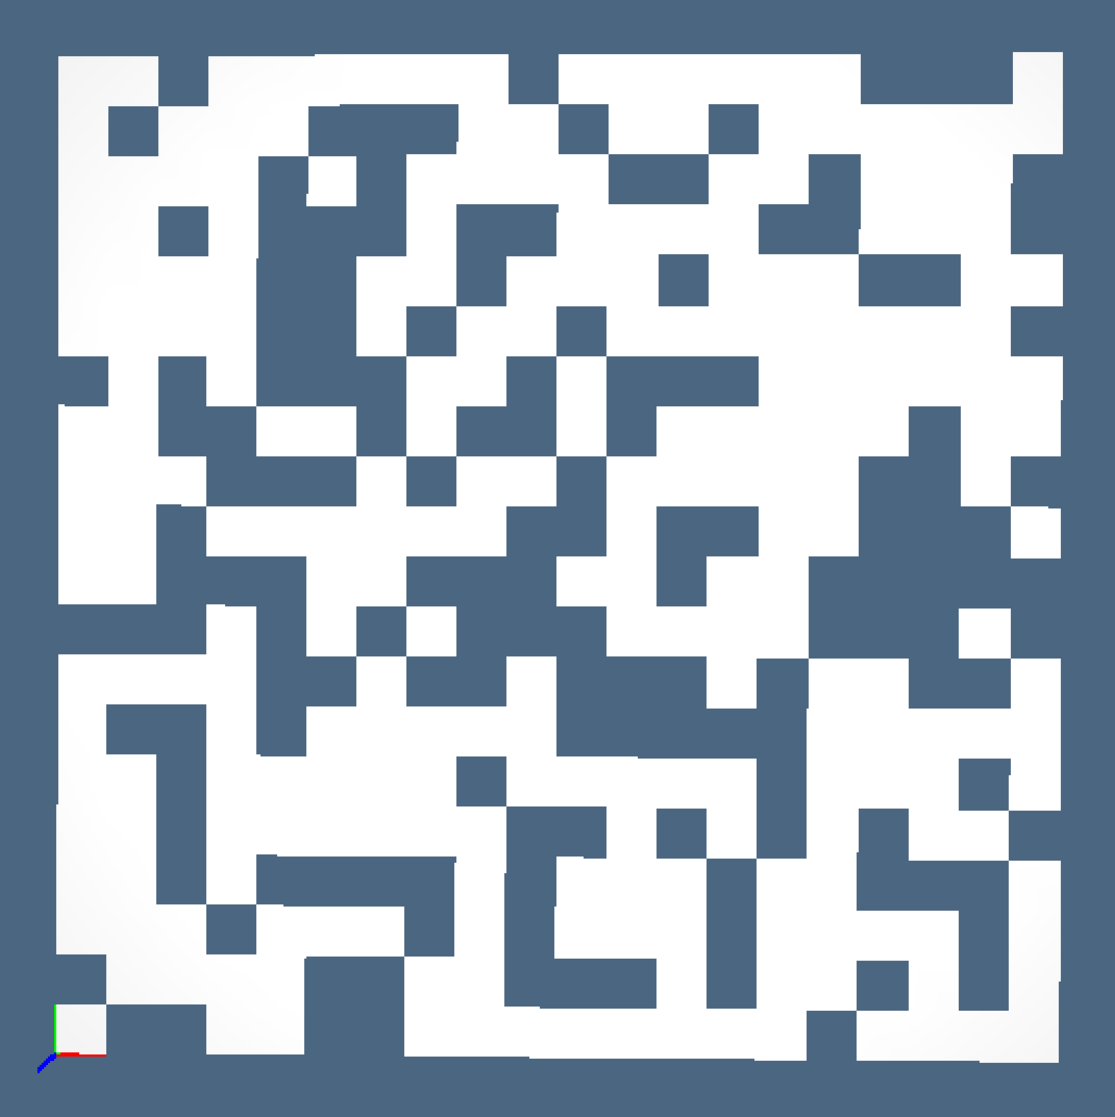
\includegraphics[height=0.243\linewidth,width=0.243\linewidth]{images/zigzag1} 
   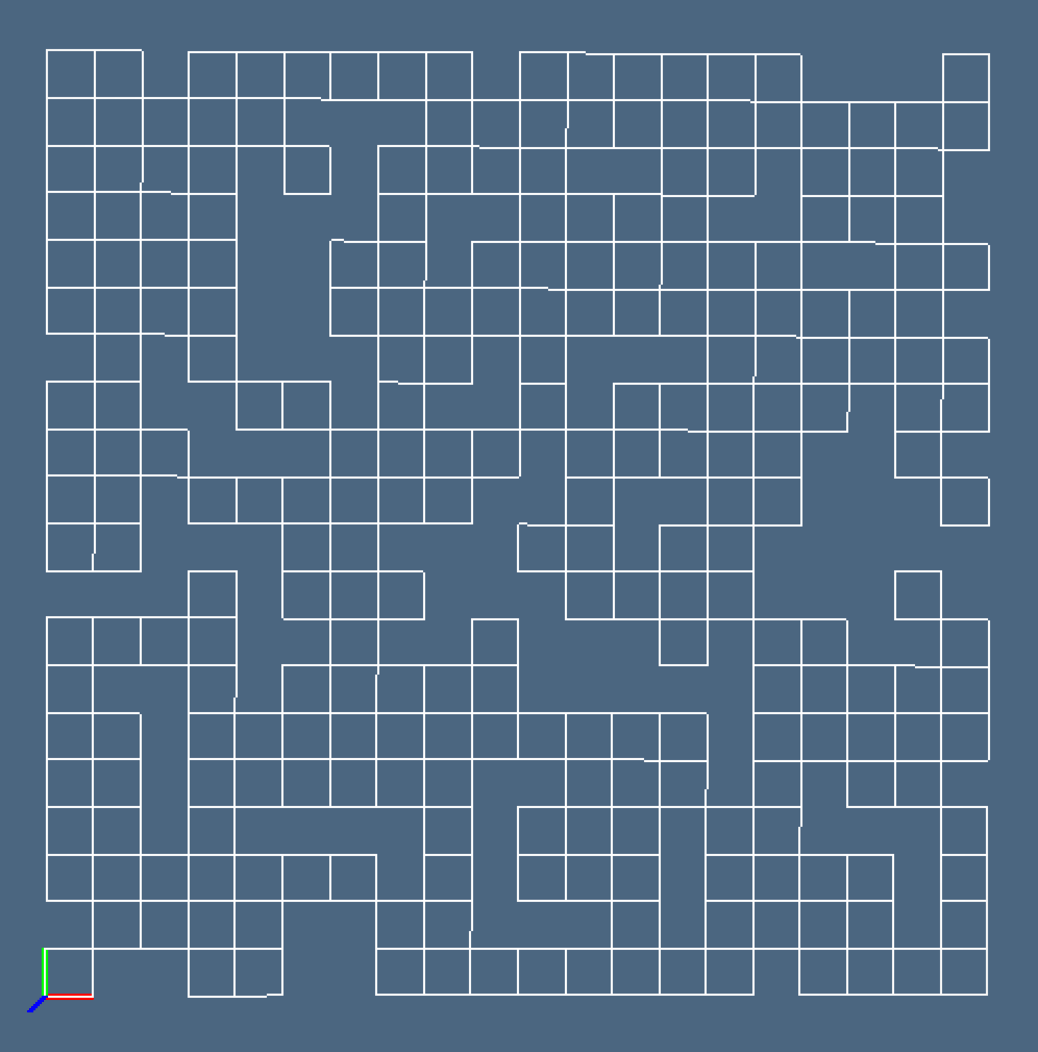
\includegraphics[height=0.243\linewidth,width=0.243\linewidth]{images/zigzag2} 
   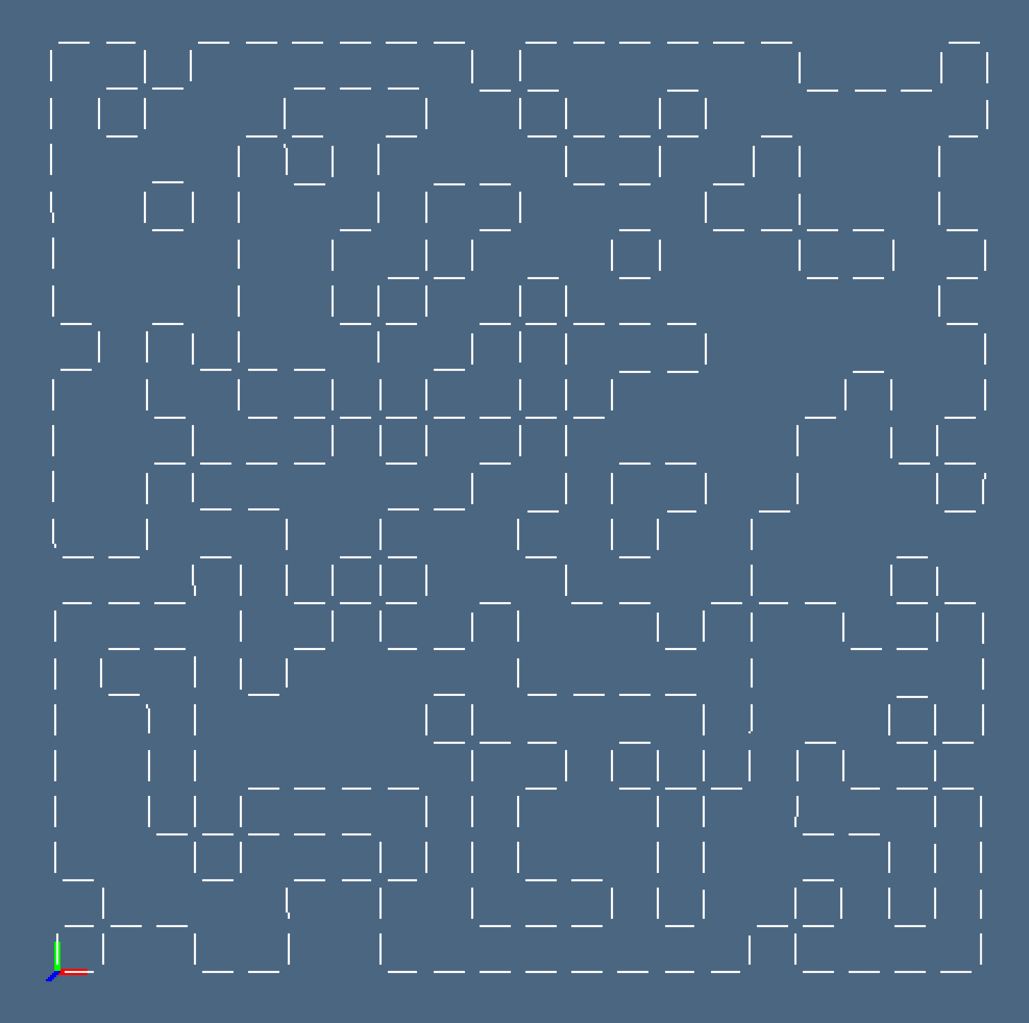
\includegraphics[height=0.243\linewidth,width=0.243\linewidth]{images/zigzag3} 
   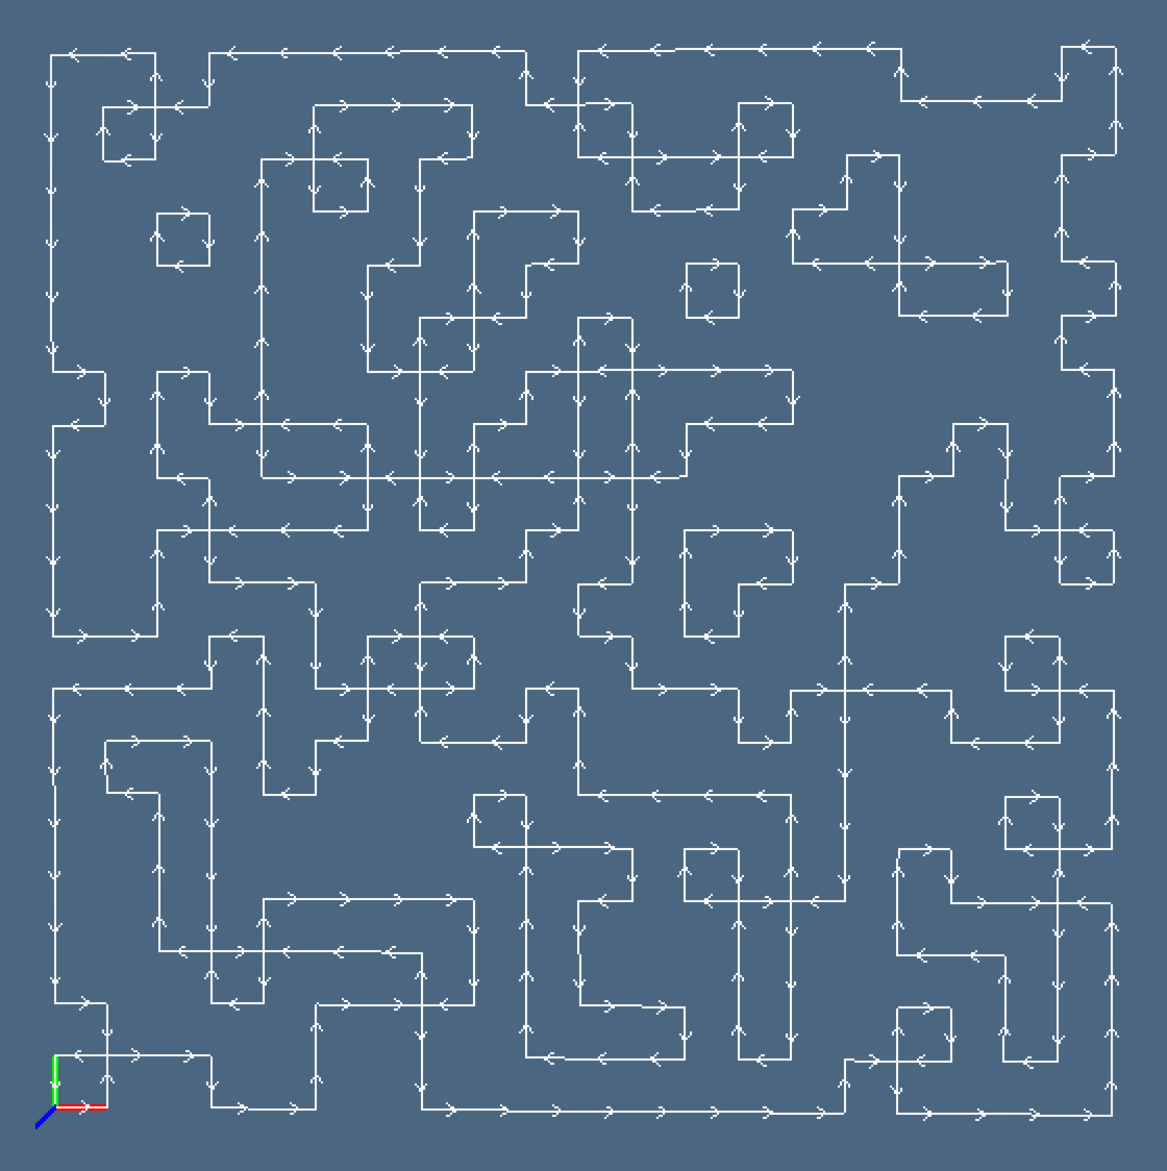
\includegraphics[height=0.243\linewidth,width=0.243\linewidth]{images/zigzag4} 
   \caption{The orientation of the boundary of a random cuboidal 2-complex;
   (a) 2-cells; (b) 1-cells; (c) exploded boundary 1-chain; (d) oriented boundary 1-chain.}
   \label{zigzag}
\vspace{5mm}
   \centering
   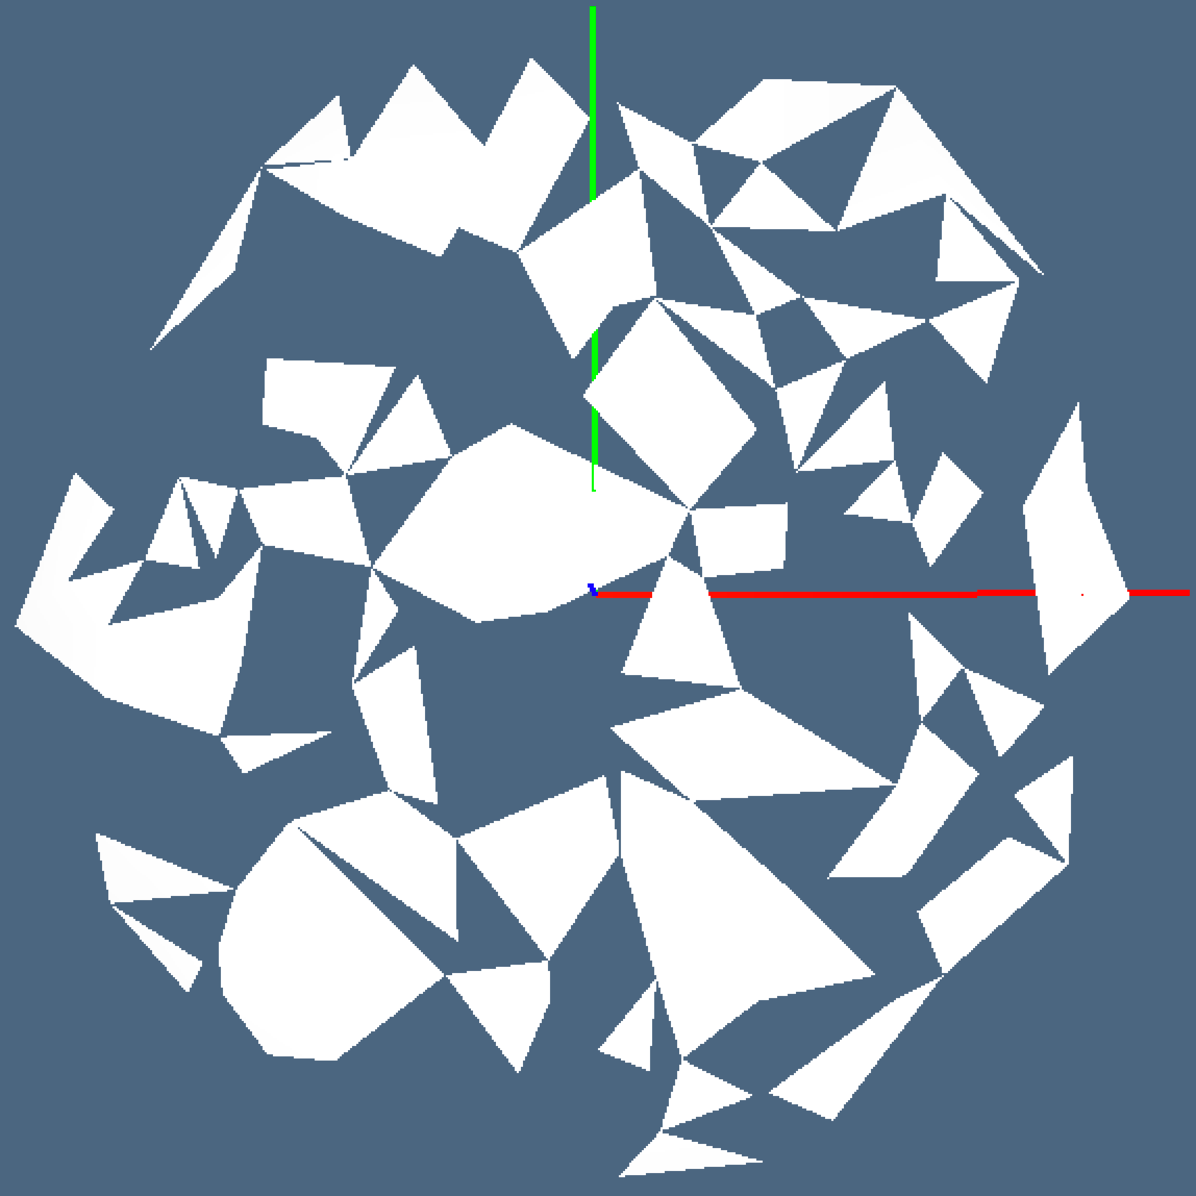
\includegraphics[height=0.328\linewidth,width=0.328\linewidth]{images/randomdelaunay1} 
   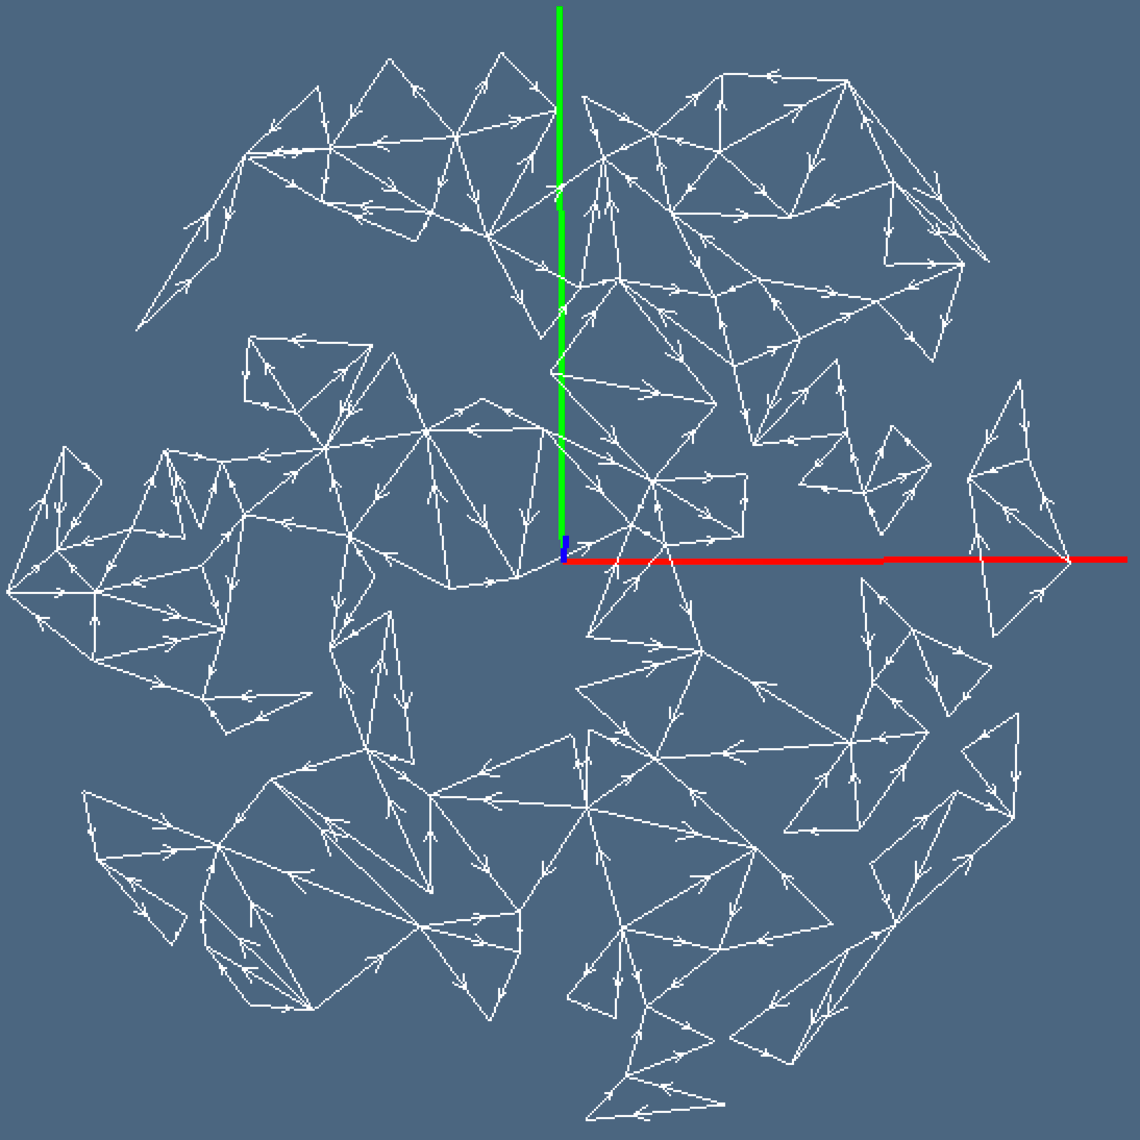
\includegraphics[height=0.328\linewidth,width=0.328\linewidth]{images/randomdelaunay2} 
   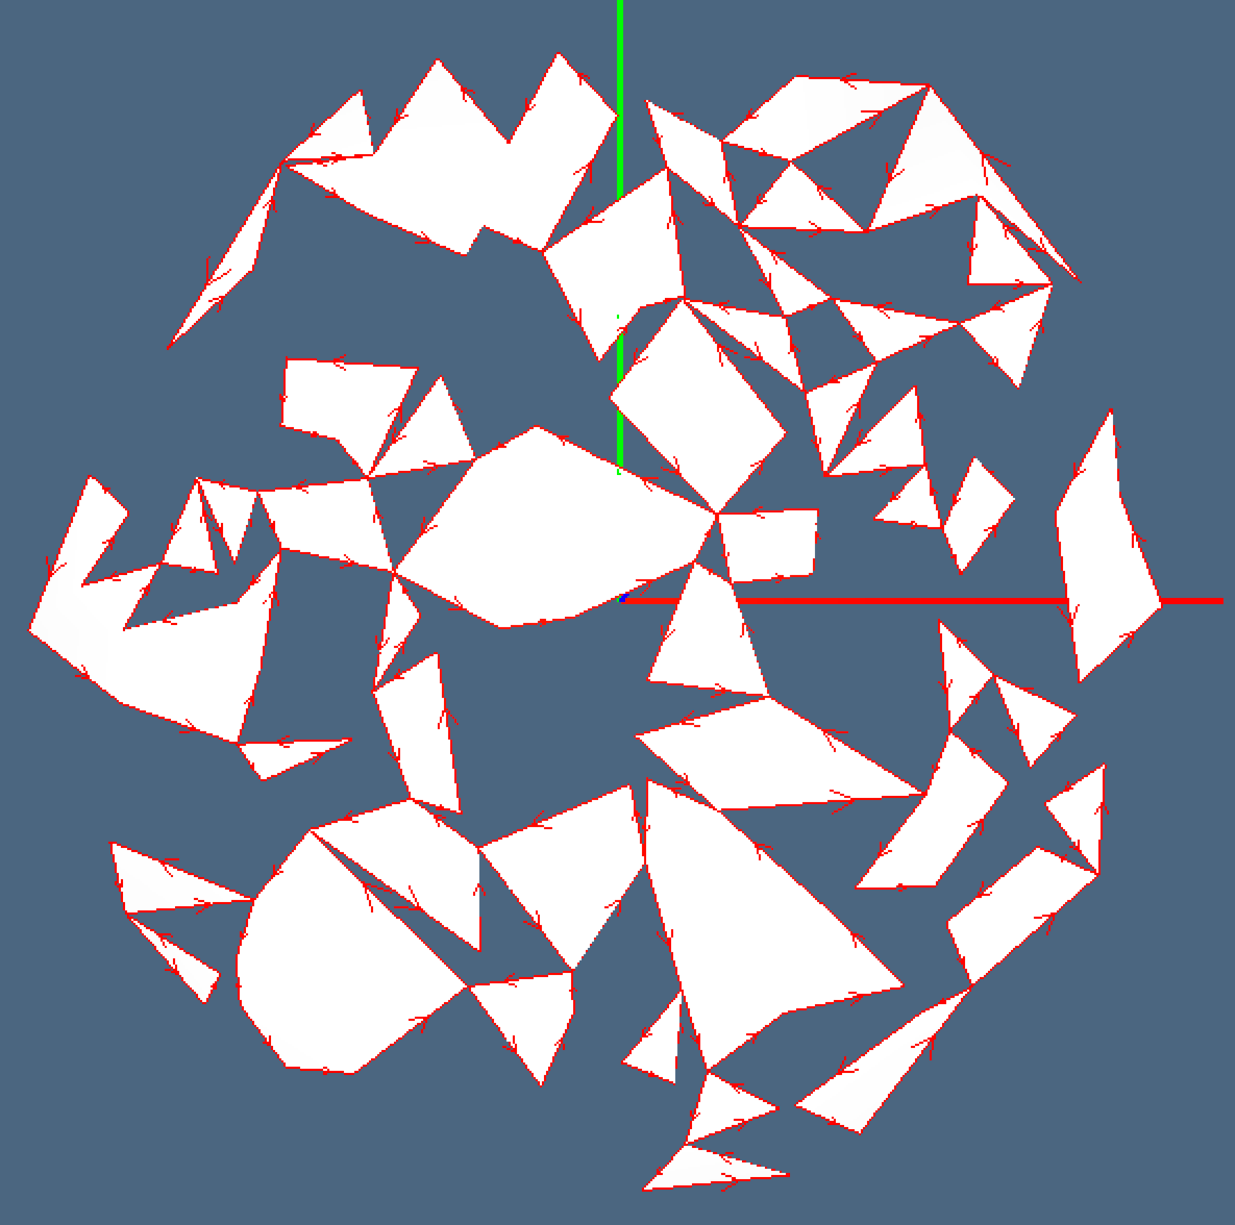
\includegraphics[height=0.328\linewidth,width=0.328\linewidth]{images/randomdelaunay3} 
   \caption{The orientation of the boundary of a random simplicial 2-complex;
   (a) 2-cells; (b) 1-cells; (c) oriented boundary 1-chain (red).}
   \label{randomdelaunay}
\end{figure}


\paragraph{Top-down implementation}

%-------------------------------------------------------------------------------
@O test/py/larcc/test16.py
@{""" Boundary orientation of a random 2D triangulation """
import sys;sys.path.insert(0, 'lib/py/')
from scipy import linalg
from larcc import *
from random import random

@< Vertices V generated as random point in the unit circle @>
@< Delaunay triangulation of the whole set V of points @>
@< Fraction of triangles randomly discarded @>
@< Coherently orient the input LAR model (V,FV)  @>
@< Compute the 1-cell and 0-cell bases EV and VV @>
@< Signed 2-boundary matrix and signed boundary 1-chain @>	
@< Display the boundary 1-chain @>
@}
%-------------------------------------------------------------------------------

\paragraph{Vertices V generated as random point in the unit circle}
%-------------------------------------------------------------------------------
@D Vertices V generated as random point in the unit circle
@{""" Vertices V generated as random point in the unit circle """
verts = []
npoints = 200
for k in range(npoints):
	t = 2*pi*random()
	u = random()+random()
	if u > 1: r = 2-u 
	else: r = u
	verts += [[r*cos(t), r*sin(t)]]
VIEW(STRUCT(AA(MK)(verts)))
@}
%-------------------------------------------------------------------------------

\paragraph{Delaunay triangulation of the whole set V of points}
%-------------------------------------------------------------------------------
@D Delaunay triangulation of the whole set V of points
@{""" Delaunay triangulation of the whole set V of points """
triangles = Delaunay(verts)
def area(cell): return linalg.det([verts[v]+[1] for v in cell])/2
cells = [ cell for cell in triangles.vertices.tolist() if area(cell)>PI/(3*npoints)]
V, FV = AA(list)(verts), cells
@}
%-------------------------------------------------------------------------------

\paragraph{Fraction of triangles randomly discarded}
%-------------------------------------------------------------------------------
@D Fraction of triangles randomly discarded
@{""" Fraction of triangles randomly discarded """
fraction = 0.7
cellSpan = len(FV)
remove = [int(random()*cellSpan) for k in range(int(cellSpan*fraction)) ]
FV = [FV[k] for k in range(cellSpan) if not k in remove]
@}
%-------------------------------------------------------------------------------

\paragraph{Coherent orientation of input LAR model (V,FV)}
%-------------------------------------------------------------------------------
@D Coherently orient the input LAR model (V,FV)
@{""" Coherently orient the input LAR model (V,FV) """
def positiveOrientation(model):
	V,simplices = model
	out = []
	for simplex in simplices:
		theMat = [V[v]+[1] for v in simplex]
		if sign(linalg.det(theMat)) > 0:  out += [simplex]
		else: out += [REVERSE(simplex)]
	return V,out

V,FV = positiveOrientation((V,FV))
@}
%-------------------------------------------------------------------------------

\paragraph{Compute the 1-cell and 0-cell bases EV and VV}
%-------------------------------------------------------------------------------
@D Compute the 1-cell and 0-cell bases EV and VV
@{""" Compute the 1-cell and 0-cell bases EV and VV """
EV = larSimplexFacets(FV)
VV = AA(LIST)(range(len(V)))
VIEW(mkSignedEdges((V,EV)))
@}
%-------------------------------------------------------------------------------

\paragraph{Signed boundary matrix [$\partial_2$] and signed boundary 1-chain}
%-------------------------------------------------------------------------------
@D Signed 2-boundary matrix and signed boundary 1-chain
@{""" Signed 2-boundary matrix  and signed boundary 1-chain """
orientedBoundary = signedCellularBoundaryCells(V,[VV,EV,FV])
cells = [EV[e] if sign==1 else REVERSE(EV[e]) for (sign,e) in zip(*orientedBoundary)]
@}
%-------------------------------------------------------------------------------

\paragraph{Display the boundary 1-chain}
%-------------------------------------------------------------------------------
@D Display the boundary 1-chain
@{""" Display the boundary 1-chain """
VIEW(STRUCT(MKPOLS((V,FV))))
VIEW(STRUCT(
	MKPOLS((V,FV)) +
	[COLOR(RED)(mkSignedEdges((V,cells)))]  ))
@}
%-------------------------------------------------------------------------------


%-------------------------------------------------------------------------------

\subsection{Orienting polytopal cells}

An orientation can be allocated to a general convex (polytopal) cell by computing the biggest simplex in its interior, and attributing to the cell the orientation of the contained simplex. 
It is in fact easy to see that the orientation can be propagated via adjacent coherently oriented simplexes, until to cover the whole cell.

The variables in the following script have the meaning specified below:
{input} :  "cell" indices of a convex and solid polytopes and "V" vertices;
{output} :  biggest "simplex" indices spanning the polytope;
{\tt m} : number of cell vertices;
{\tt d} : dimension (number of coordinates) of cell vertices;
{\tt d+1} : number of simplex vertices;
{\tt vcell} : cell vertices;
{\tt vsimplex} : simplex vertices;
{\tt Id} : identity matrix;
{\tt basis} : orthonormal spanning set of vectors $e_k$;
{\tt vector} : position vector of a simplex vertex in translated coordinates;
{\tt unUsedIndices} : cell indices not moved to simplex.

%-------------------------------------------------------------------------------
@D Oriented boundary cells for simplicial models
@{def pivotSimplices(V,CV,d=3):
	simplices = []
	for cell in CV:
		vcell = np.array([V[v] for v in cell])
		m, simplex = len(cell), []
		# translate the cell: for each k, vcell[k] -= vcell[0], and simplex[0] := cell[0]
		for k in range(m-1,-1,-1): vcell[k] -= vcell[0]
		# simplex = [0], basis = [], tensor = Id(d+1)
		simplex += [cell[0]]
		basis = []
		tensor = np.array(IDNT(d))
		# look for most distant cell vertex
		dists = [SUM([SQR(x) for x in v])**0.5 for v in vcell]
		maxDistIndex = max(enumerate(dists),key=lambda x: x[1])[0]
		vector = np.array([vcell[maxDistIndex]])
		# normalize vector
		den=(vector**2).sum(axis=-1) **0.5
		basis = [vector/den]
		simplex += [cell[maxDistIndex]]
		unUsedIndices = [h for h in cell if h not in simplex]
		
		# for k in {2,d+1}:
		for k in range(2,d+1):
			# update the orthonormal tensor
			e = basis[-1]
			tensor = tensor - np.dot(e.T, e)
			# compute the index h of a best vector
			# look for most distant cell vertex
			dists = [SUM([SQR(x) for x in np.dot(tensor,v)])**0.5
			if h in unUsedIndices else 0.0
			for (h,v) in zip(cell,vcell)]
			# insert the best vector index h in output simplex
			maxDistIndex = max(enumerate(dists),key=lambda x: x[1])[0]
			vector = np.array([vcell[maxDistIndex]])
			# normalize vector
			den=(vector**2).sum(axis=-1) **0.5
			basis += [vector/den]
			simplex += [cell[maxDistIndex]]
			unUsedIndices = [h for h in cell if h not in simplex]
		simplices += [simplex]
	return simplices

def simplexOrientations(V,simplices):
	vcells = [[V[v]+[1.0] for v in simplex] for simplex in simplices]
	return [SIGN(np.linalg.det(vcell)) for vcell in vcells]
@}
%-------------------------------------------------------------------------------



\section{Exporting the library}

\subsection{MIT licence}
%-------------------------------------------------------------------------------
@D The MIT Licence
@{
"""
The MIT License
===============
	
Permission is hereby granted, free of charge, to any person obtaining
a copy of this software and associated documentation files (the
'Software'), to deal in the Software without restriction, including
without limitation the rights to use, copy, modify, merge, publish,
distribute, sublicense, and/or sell copies of the Software, and to
permit persons to whom the Software is furnished to do so, subject to
the following conditions:

The above copyright notice and this permission notice shall be
included in all copies or substantial portions of the Software.

THE SOFTWARE IS PROVIDED 'AS IS', WITHOUT WARRANTY OF ANY KIND,
EXPRESS OR IMPLIED, INCLUDING BUT NOT LIMITED TO THE WARRANTIES OF
MERCHANTABILITY, FITNESS FOR A PARTICULAR PURPOSE AND NONINFRINGEMENT.
IN NO EVENT SHALL THE AUTHORS OR COPYRIGHT HOLDERS BE LIABLE FOR ANY
CLAIM, DAMAGES OR OTHER LIABILITY, WHETHER IN AN ACTION OF CONTRACT,
TORT OR OTHERWISE, ARISING FROM, OUT OF OR IN CONNECTION WITH THE
SOFTWARE OR THE USE OR OTHER DEALINGS IN THE SOFTWARE.
"""
@}
%-------------------------------------------------------------------------------
\subsection{Importing of modules or packages}
%-------------------------------------------------------------------------------
@D Importing of modules or packages
@{from pyplasm import *
import collections
import scipy
import numpy as np
from scipy import zeros,arange,mat,amin,amax,array
from scipy.sparse import vstack,hstack,csr_matrix,coo_matrix,lil_matrix,triu

from lar2psm import *
from sysml import *
@}
%-------------------------------------------------------------------------------

\subsection{Writing the library file}

%-------------------------------------------------------------------------------
@o lib/py/larcc.py
@{# -*- coding: utf-8 -*-
""" Basic LARCC library """
@< The MIT Licence @>
@< Importing of modules or packages @>
@< From list of triples to scipy.sparse @>
@< Brc to Coo transformation @>
@< Coo to Csr transformation @>
@< Brc to Csr transformation @>
@< Query Matrix shape @>
@< Sparse to dense matrix transformation @>
@< Matrix product and transposition @>
@< Matrix filtering to produce the boundary matrix @>
@< Matrix filtering via a generic predicate @>
@< From cells and facets to boundary operator @>
@< From cells and facets to boundary cells @>
@< Signed boundary matrix for simplicial models @>
@< Orientation of general convex cells @>
@< Computation of cell adjacencies @>
@< Extraction of facets of a cell complex @>
@< Some incidence operators @>
@< Visualization of cell indices @>
@< Numbered visualization of a LAR model @>
@< Drawing of oriented edges @>
@< Incidence chain computation @>
@< Signed boundary matrix for polytopal complexes @>
@< Signed boundary cells for polytopal complexes @>
@<  Oriented boundary cells for simplicial models @>

if __name__ == "__main__": 
	@< Test examples @>
@}
%-------------------------------------------------------------------------------

\section{Unit tests}


%-------------------------------------------------------------------------------
@D Test examples
@{
@< Test example of Brc to Coo transformation @>
@< Test example of Coo to Csr transformation @>
@< Test example of Brc to Csr transformation @>
@< Test examples of Query Matrix shape @>
@< Test examples of Sparse to dense matrix transformation @>
@< Test example of Matrix filtering to produce the boundary matrix @>
@< Test example of Matrix filtering via a generic predicate @>
@< Test examples of From cells and facets to boundary operator @>
@< Test examples of From cells and facets to boundary cells @>
@< Test examples of Computation of cell adjacencies @>
@< Test examples of Extraction of facets of a cell complex @>
@}
%-------------------------------------------------------------------------------

\paragraph{Comparing oriented and unoriented boundary}

%-------------------------------------------------------------------------------
@O test/py/larcc/test09.py
@{""" comparing oriented boundary and unoriented boundary extraction on a simple example """
import sys; sys.path.insert(0, 'lib/py/')
from largrid import *
from larcc import *

V,CV = larSimplexGrid1([1,1,1])
FV = larSimplexFacets(CV)

orientedBoundary = signedBoundaryCells(V,CV,FV)
orientedBoundaryFV = [FV[-k] if k<0 else swap(FV[k]) for k in orientedBoundary]
VIEW(EXPLODE(1.5,1.5,1.5)(MKPOLS((V,orientedBoundaryFV))))

BF = boundaryCells(CV,FV)
boundaryCellsFV = [FV[k] for k in BF]
VIEW(EXPLODE(1.5,1.5,1.5)(MKPOLS((V,boundaryCellsFV))))
@}
%-------------------------------------------------------------------------------

%-------------------------------------------------------------------------------
@O test/py/larcc/test12.py
@{""" comparing edge orientation and oriented boundary extraction """
import sys; sys.path.insert(0, 'lib/py/')
from largrid import *
from larcc import *

V,FV = larSimplexGrid1([5,5])
EV = larSimplexFacets(FV)
VIEW(mkSignedEdges((V,EV)))

orientedBoundary = signedBoundaryCells(V,FV,EV)
orientedBoundaryEV = [EV[-k] if k<0 else swap(EV[k]) for k in orientedBoundary]
VIEW(mkSignedEdges((V,orientedBoundaryEV)))
@}
%-------------------------------------------------------------------------------



\appendix

\section{Appendix: Tutorials}


\subsection{Model generation, skeleton and boundary extraction}

%-------------------------------------------------------------------------------
@o test/py/larcc/test01.py
@{import sys; sys.path.insert(0, 'lib/py/')
from larcc import *
from largrid import *
@< input of 2D topology and geometry data @>
@< characteristic matrices @>
@< incidence matrix @>
@< boundary and coboundary operators @>
@< product of cell complexes @>
@< 2-skeleton extraction @>
@< 1-skeleton extraction  @>
@< 0-coboundary computation @>
@< 1-coboundary computation @>
@< 2-coboundary computation @>
@< boundary chain visualisation @>
@}
%-------------------------------------------------------------------------------

%-------------------------------------------------------------------------------
@D input of 2D topology and geometry data
@{
# input of geometry and topology  
V2 = [[4,10],[8,10],[14,10],[8,7],[14,7],[4,4],[8,4],[14,4]]
EV = [[0,1],[1,2],[3,4],[5,6],[6,7],[0,5],[1,3],[2,4],[3,6],[4,7]]
FV = [[0,1,3,5,6],[1,2,3,4],[3,4,6,7]]
@}
%-------------------------------------------------------------------------------

%-------------------------------------------------------------------------------
@D characteristic matrices
@{# characteristic matrices
csrFV = csrCreate(FV)
csrEV = csrCreate(EV)
print "\nFV =\n", csr2DenseMatrix(csrFV)
print "\nEV =\n", csr2DenseMatrix(csrEV)
@}
%-------------------------------------------------------------------------------

%-------------------------------------------------------------------------------
@D incidence matrix
@{# product
csrEF = matrixProduct(csrEV, csrTranspose(csrFV))
print "\nEF =\n", csr2DenseMatrix(csrEF)
@}
%-------------------------------------------------------------------------------

%-------------------------------------------------------------------------------
@D boundary and coboundary operators
@{# boundary and coboundary operators
facetLengths = [csrCell.getnnz() for csrCell in csrEV]
boundary = csrBoundaryFilter(csrEF,facetLengths)
coboundary_1 = csrTranspose(boundary)
print "\ncoboundary_1 =\n", csr2DenseMatrix(coboundary_1)
@}
%-------------------------------------------------------------------------------

%-------------------------------------------------------------------------------
@D product of cell complexes
@{# product operator
mod_2D = (V2,FV)
V1,topol_0 = [[0.],[1.],[2.]], [[0],[1],[2]]
topol_1 = [[0,1],[1,2]]
mod_0D = (V1,topol_0)
mod_1D = (V1,topol_1)
V3,CV = larModelProduct([mod_2D,mod_1D])
mod_3D = (V3,CV)
VIEW(EXPLODE(1.2,1.2,1.2)(MKPOLS(mod_3D)))
print "\nk_3 =", len(CV), "\n"
@}
%-------------------------------------------------------------------------------

%-------------------------------------------------------------------------------
@D 2-skeleton extraction
@{# 2-skeleton of the 3D product complex
mod_2D_1 = (V2,EV)
mod_3D_h2 = larModelProduct([mod_2D,mod_0D])
mod_3D_v2 = larModelProduct([mod_2D_1,mod_1D])
_,FV_h = mod_3D_h2
_,FV_v = mod_3D_v2
FV3 = FV_h + FV_v
SK2 = (V3,FV3)
VIEW(EXPLODE(1.2,1.2,1.2)(MKPOLS(SK2)))
print "\nk_2 =", len(FV3), "\n"
@}
%-------------------------------------------------------------------------------

%-------------------------------------------------------------------------------
@D 1-skeleton extraction 
@{# 1-skeleton of the 3D product complex 
mod_2D_0 = (V2,AA(LIST)(range(len(V2))))
mod_3D_h1 = larModelProduct([mod_2D_1,mod_0D])
mod_3D_v1 = larModelProduct([mod_2D_0,mod_1D])
_,EV_h = mod_3D_h1
_,EV_v = mod_3D_v1
EV3 = EV_h + EV_v
SK1 = (V3,EV3)
VIEW(EXPLODE(1.2,1.2,1.2)(MKPOLS(SK1)))
print "\nk_1 =", len(EV3), "\n"
@}
%-------------------------------------------------------------------------------

%-------------------------------------------------------------------------------
@D 0-coboundary computation
@{# boundary and coboundary operators
np.set_printoptions(threshold=sys.maxint)
csrFV3 = csrCreate(FV3)
csrEV3 = csrCreate(EV3)
csrVE3 = csrTranspose(csrEV3)
facetLengths = [csrCell.getnnz() for csrCell in csrEV3]
boundary = csrBoundaryFilter(csrVE3,facetLengths)
coboundary_0 = csrTranspose(boundary)
print "\ncoboundary_0 =\n", csr2DenseMatrix(coboundary_0)
@}
%-------------------------------------------------------------------------------

%-------------------------------------------------------------------------------
@D 1-coboundary computation
@{csrEF3 = matrixProduct(csrEV3, csrTranspose(csrFV3))
facetLengths = [csrCell.getnnz() for csrCell in csrFV3]
boundary = csrBoundaryFilter(csrEF3,facetLengths)
coboundary_1 = csrTranspose(boundary)
print "\ncoboundary_1.T =\n", csr2DenseMatrix(coboundary_1.T)
@}
%-------------------------------------------------------------------------------

%-------------------------------------------------------------------------------
@D 2-coboundary computation
@{csrCV = csrCreate(CV)
csrFC3 = matrixProduct(csrFV3, csrTranspose(csrCV))
facetLengths = [csrCell.getnnz() for csrCell in csrCV]
boundary = csrBoundaryFilter(csrFC3,facetLengths)
coboundary_2 = csrTranspose(boundary)
print "\ncoboundary_2 =\n", csr2DenseMatrix(coboundary_2)
@}
%-------------------------------------------------------------------------------

%-------------------------------------------------------------------------------
@D boundary chain visualisation
@{# boundary chain visualisation
boundaryCells_2 = boundaryCells(CV,FV3)
boundary = (V3,[FV3[k] for k in boundaryCells_2])
VIEW(EXPLODE(1.5,1.5,1.5)(MKPOLS(boundary)))
@}
%-------------------------------------------------------------------------------



\subsection{Boundary of 3D simplicial grid}

%-------------------------------------------------------------------------------
@o test/py/larcc/test02.py
@{import sys; sys.path.insert(0, 'lib/py/')
@< boundary of 3D simplicial grid @>
@}
%-------------------------------------------------------------------------------

%-------------------------------------------------------------------------------
@D boundary of 3D simplicial grid
@{from simplexn import *
from larcc import *

V,CV = larSimplexGrid1([10,10,3])
VIEW(EXPLODE(1.5,1.5,1.5)(MKPOLS((V,CV))))
SK2 = (V,larSimplexFacets(CV))
VIEW(EXPLODE(1.5,1.5,1.5)(MKPOLS(SK2)))
_,FV = SK2
SK1 = (V,larSimplexFacets(FV))
_,EV = SK1
VIEW(EXPLODE(1.5,1.5,1.5)(MKPOLS(SK1)))

boundaryCells_2 = boundaryCells(CV,FV)
boundary = (V,[FV[k] for k in boundaryCells_2])
VIEW(EXPLODE(1.5,1.5,1.5)(MKPOLS(boundary)))
print "\nboundaryCells_2 =\n", boundaryCells_2

boundaryCells_2 = signedBoundaryCells(V,CV,FV)
boundaryFV = [FV[-k] if k<0 else swap(FV[k]) for k in boundaryCells_2]

VIEW(EXPLODE(1.5,1.5,1.5)(MKPOLS((V,boundaryFV))))
print "\nboundaryCells_2 =\n", boundaryFV
@}
%-------------------------------------------------------------------------------


\subsection{Oriented boundary of a random simplicial complex}


%-------------------------------------------------------------------------------
@o test/py/larcc/test03.py
@{@< Importing external modules @>
@< Generating and viewing a random 3D simplicial complex @>
@< Computing and viewing its non-oriented boundary @>
@< Computing and viewing its oriented boundary @>
@}
%-------------------------------------------------------------------------------


%-------------------------------------------------------------------------------
@D Importing external modules
@{import sys; sys.path.insert(0, 'lib/py/')
from simplexn import *
from larcc import *
from scipy import *
from scipy.spatial import Delaunay
import numpy as np
@}
%-------------------------------------------------------------------------------

%-------------------------------------------------------------------------------
@D Generating and viewing a random 3D simplicial complex
@{verts = np.random.rand(10000, 3) # 1000 points in 3-d
verts = [AA(lambda x: 2*x)(VECTDIFF([vert,[0.5,0.5,0.5]])) for vert in verts]
verts = [vert for vert in verts if VECTNORM(vert) < 1.0]
tetra = Delaunay(verts)
cells = [cell for cell in tetra.vertices.tolist()
		 if  ((verts[cell[0]][2]<0) and (verts[cell[1]][2]<0) 
		 		and (verts[cell[2]][2]<0) and (verts[cell[3]][2]<0) ) ]
V, CV = verts, cells
VIEW(MKPOL([V,AA(AA(lambda k:k+1))(CV),[]]))
@}
%-------------------------------------------------------------------------------

%-------------------------------------------------------------------------------
@D Computing and viewing its non-oriented boundary 
@{FV = larSimplexFacets(CV)
VIEW(MKPOL([V,AA(AA(lambda k:k+1))(FV),[]]))
boundaryCells_2 = boundaryCells(CV,FV)
print "\nboundaryCells_2 =\n", boundaryCells_2
bndry = (V,[FV[k] for k in boundaryCells_2])
VIEW(EXPLODE(1.5,1.5,1.5)(MKPOLS(bndry)))
@}
%-------------------------------------------------------------------------------

%-------------------------------------------------------------------------------
@D Computing and viewing its oriented boundary
@{boundaryCells_2 = signedBoundaryCells(V,CV,FV)
print "\nboundaryCells_2 =\n", boundaryCells_2
boundaryFV = [FV[-k] if k<0 else swap(FV[k]) for k in boundaryCells_2]
boundaryModel = (V,boundaryFV)
VIEW(EXPLODE(1.5,1.5,1.5)(MKPOLS(boundaryModel)))
@}
%-------------------------------------------------------------------------------

\subsection{Oriented boundary of a simplicial grid}

%-------------------------------------------------------------------------------
@o test/py/larcc/test04.py
@{@< Generate and view a 3D simplicial grid @>
@< Computing and viewing the 2-skeleton of simplicial grid @>
@< Computing and viewing the oriented boundary of simplicial grid @>
@}
%-------------------------------------------------------------------------------


%-------------------------------------------------------------------------------
@D Generate and view a 3D simplicial grid
@{import sys; sys.path.insert(0, 'lib/py/')
from simplexn import *
from larcc import *
V,CV = larSimplexGrid1([4,4,4])
VIEW(EXPLODE(1.5,1.5,1.5)(MKPOLS((V,CV))))
@}
%-------------------------------------------------------------------------------

%-------------------------------------------------------------------------------
@D Computing and viewing the 2-skeleton of simplicial grid
@{FV = larSimplexFacets(CV)
EV = larSimplexFacets(FV)
VIEW(EXPLODE(1.5,1.5,1.5)(MKPOLS((V,FV))))
@}
%-------------------------------------------------------------------------------

%-------------------------------------------------------------------------------
@D Computing and viewing the oriented boundary of simplicial grid
@{csrSignedBoundaryMat = signedSimplicialBoundary (CV,FV)
boundaryCells_2 = signedBoundaryCells(V,CV,FV)
boundaryFV = [FV[-k] if k<0 else swap(FV[k]) for k in boundaryCells_2]
boundary = (V,boundaryFV)
VIEW(EXPLODE(1.5,1.5,1.5)(MKPOLS(boundary)))
@}
%-------------------------------------------------------------------------------


\subsection{Skeletons and oriented boundary of a simplicial complex}


%-------------------------------------------------------------------------------
@o test/py/larcc/test05.py
@{import sys; sys.path.insert(0, 'lib/py/')

@< Skeletons computation and vilualisation @>
@< Oriented boundary matrix visualization @>
@< Computation of oriented boundary cells @>
@}
%-------------------------------------------------------------------------------


%-------------------------------------------------------------------------------
@D Skeletons computation and vilualisation
@{from simplexn import *
from larcc import *
V,FV = larSimplexGrid1([3,3])
VIEW(EXPLODE(1.5,1.5,1.5)(MKPOLS((V,FV))))
EV = larSimplexFacets(FV)
VIEW(EXPLODE(1.5,1.5,1.5)(MKPOLS((V,EV))))
VV = larSimplexFacets(EV)
VIEW(EXPLODE(1.5,1.5,1.5)(MKPOLS((V,VV))))
@}
%-------------------------------------------------------------------------------

%-------------------------------------------------------------------------------
@D Oriented boundary matrix visualization
@{np.set_printoptions(threshold='nan')
csrSignedBoundaryMat = signedSimplicialBoundary (FV,EV)
Z = csr2DenseMatrix(csrSignedBoundaryMat)
print "\ncsrSignedBoundaryMat =\n", Z
from pylab import *
matshow(Z)
show()
@}
%-------------------------------------------------------------------------------

%-------------------------------------------------------------------------------
@D Computation of oriented boundary cells 
@{boundaryCells_1 = signedBoundaryCells(V,FV,EV)
print "\nboundaryCells_1 =\n", boundaryCells_1
boundaryEV = [EV[-k] if k<0 else swap(EV[k]) for k in boundaryCells_1]
bndry = (V,boundaryEV)
VIEW(EXPLODE(1.5,1.5,1.5)(MKPOLS(bndry)))
@}
%-------------------------------------------------------------------------------

\subsection{Boundary of random 2D simplicial complex}

%-------------------------------------------------------------------------------
@o test/py/larcc/test06.py
@{import sys; sys.path.insert(0, 'lib/py/')
from simplexn import *
from larcc import *
from scipy.spatial import Delaunay
@< Test for quasi-equilateral triangles @>
@< Generation and selection of random triangles @>
@< Boundary computation and visualisation @>
@}
%-------------------------------------------------------------------------------


\begin{figure}[htbp] %  figure placement: here, top, bottom, or page
   \centering
   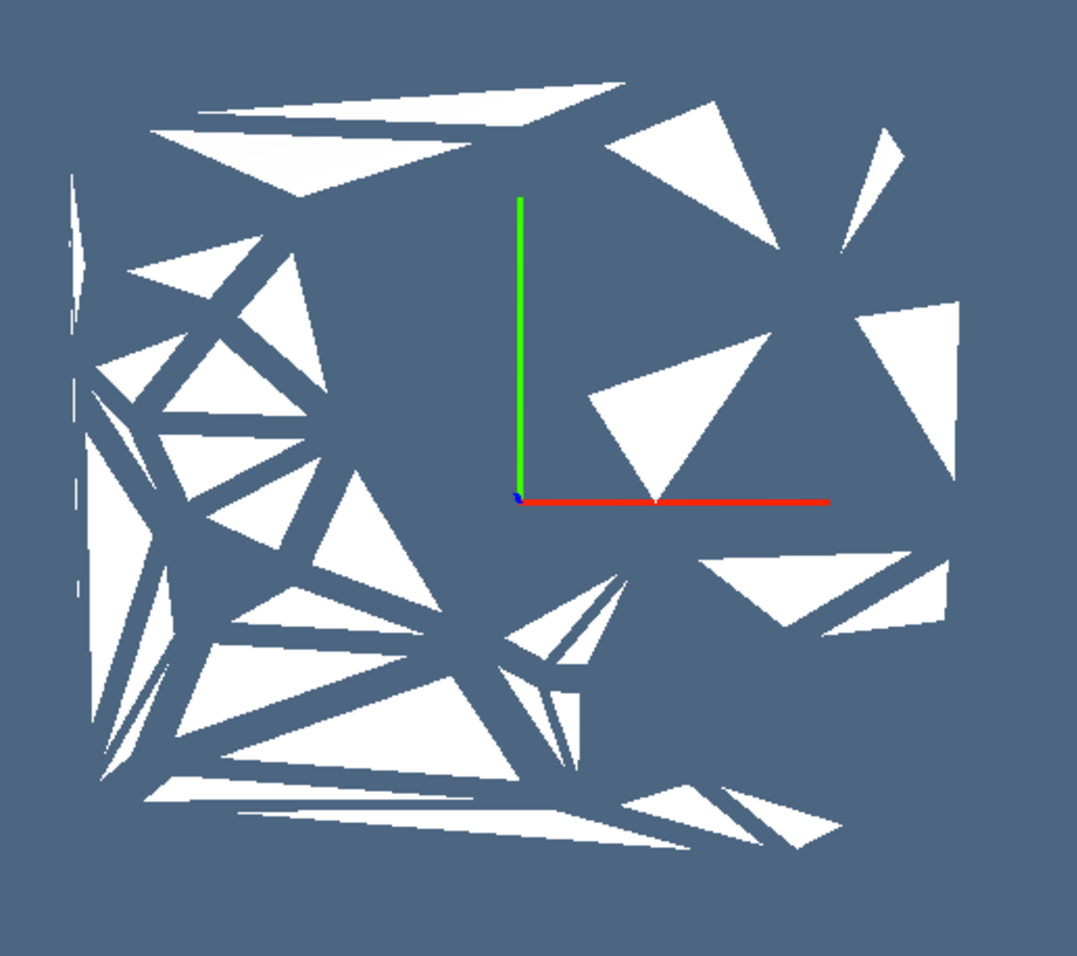
\includegraphics[height=0.25\linewidth,width=0.32\linewidth]{images/tria0} 
   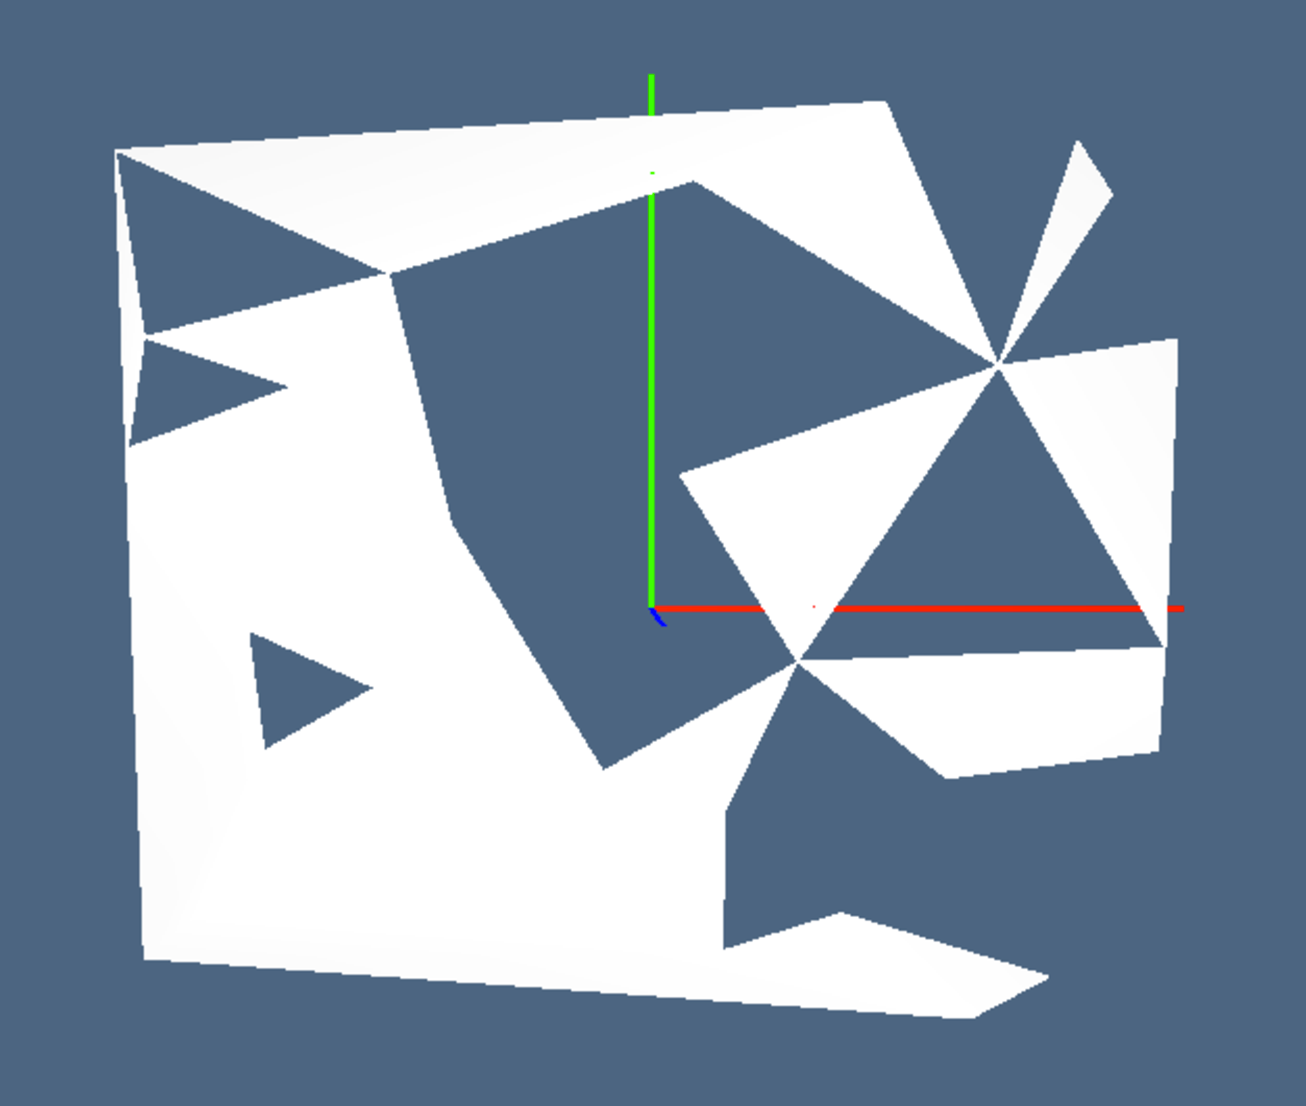
\includegraphics[height=0.25\linewidth,width=0.32\linewidth]{images/tria1} 
   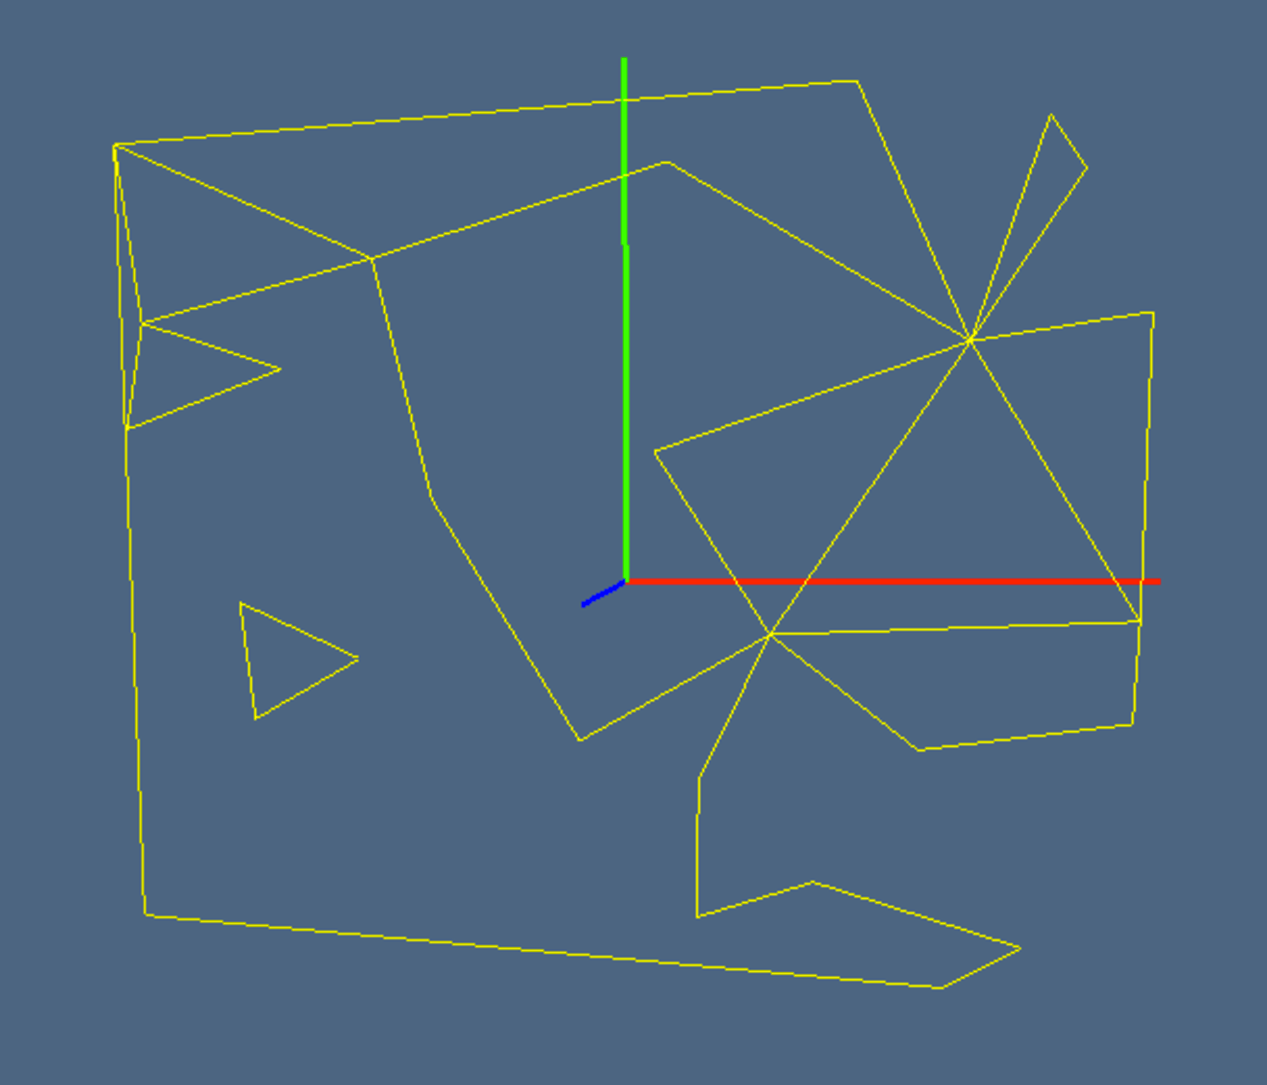
\includegraphics[height=0.25\linewidth,width=0.32\linewidth]{images/tria2} 
   \caption{example caption}
   \label{fig:example}
\end{figure}

%-------------------------------------------------------------------------------
@D Test for quasi-equilateral triangles
@{def quasiEquilateral(tria):
	a = VECTNORM(VECTDIFF(tria[0:2]))
	b = VECTNORM(VECTDIFF(tria[1:3]))
	c = VECTNORM(VECTDIFF([tria[0],tria[2]]))
	m = max(a,b,c)
	if m/a < 1.7 and m/b < 1.7 and m/c < 1.7: return True
	else: return False
@}
%-------------------------------------------------------------------------------

%-------------------------------------------------------------------------------
@D Generation and selection of random triangles 
@{verts = np.random.rand(50,2)
verts = (verts - [0.5,0.5]) * 2
triangles = Delaunay(verts)
cells = [ cell for cell in triangles.vertices.tolist()
		 if (not quasiEquilateral([verts[k] for k in cell])) ]
V, FV = AA(list)(verts), cells
EV = larSimplexFacets(FV)
pols2D = MKPOLS((V,FV))
VIEW(EXPLODE(1.5,1.5,1.5)(pols2D))
@}
%-------------------------------------------------------------------------------

%-------------------------------------------------------------------------------
@D Boundary computation and visualisation 
@{orientedBoundary = signedBoundaryCells(V,FV,EV)
submodel = mkSignedEdges((V,orientedBoundary))
VIEW(submodel)
@}
%-------------------------------------------------------------------------------


%-------------------------------------------------------------------------------
@D Decompose a permutation into cycles 
@{def permutationOrbits(List):
	d = dict((i,int(x)) for i,x in enumerate(List))
	out = []
	while d:
		x = list(d)[0]
		orbit = []
		while x in d:
			orbit += [x],
			x = d.pop(x)
		out += [CAT(orbit)+orbit[0]]
	return out
		
if __name__ == "__main__":
	print [2, 3, 4, 5, 6, 7, 0, 1]
	print permutationOrbits([2, 3, 4, 5, 6, 7, 0, 1])
	print [3,9,8,4,10,7,2,11,6,0,1,5]
	print permutationOrbits([3,9,8,4,10,7,2,11,6,0,1,5])
@}
%-------------------------------------------------------------------------------

\subsection{Assemblies of simplices and hypercubes}

%-------------------------------------------------------------------------------
@o test/py/larcc/test07.py
@{import sys; sys.path.insert(0, 'lib/py/')
from simplexn import *
from larcc import *
from largrid import *
@< Definition of 1-dimensional LAR models @>
@< Assembly generation of squares and triangles @>
@< Assembly generation  of cubes and tetrahedra @>
@}
%-------------------------------------------------------------------------------

\begin{figure}[htbp] %  figure placement: here, top, bottom, or page
   \centering
   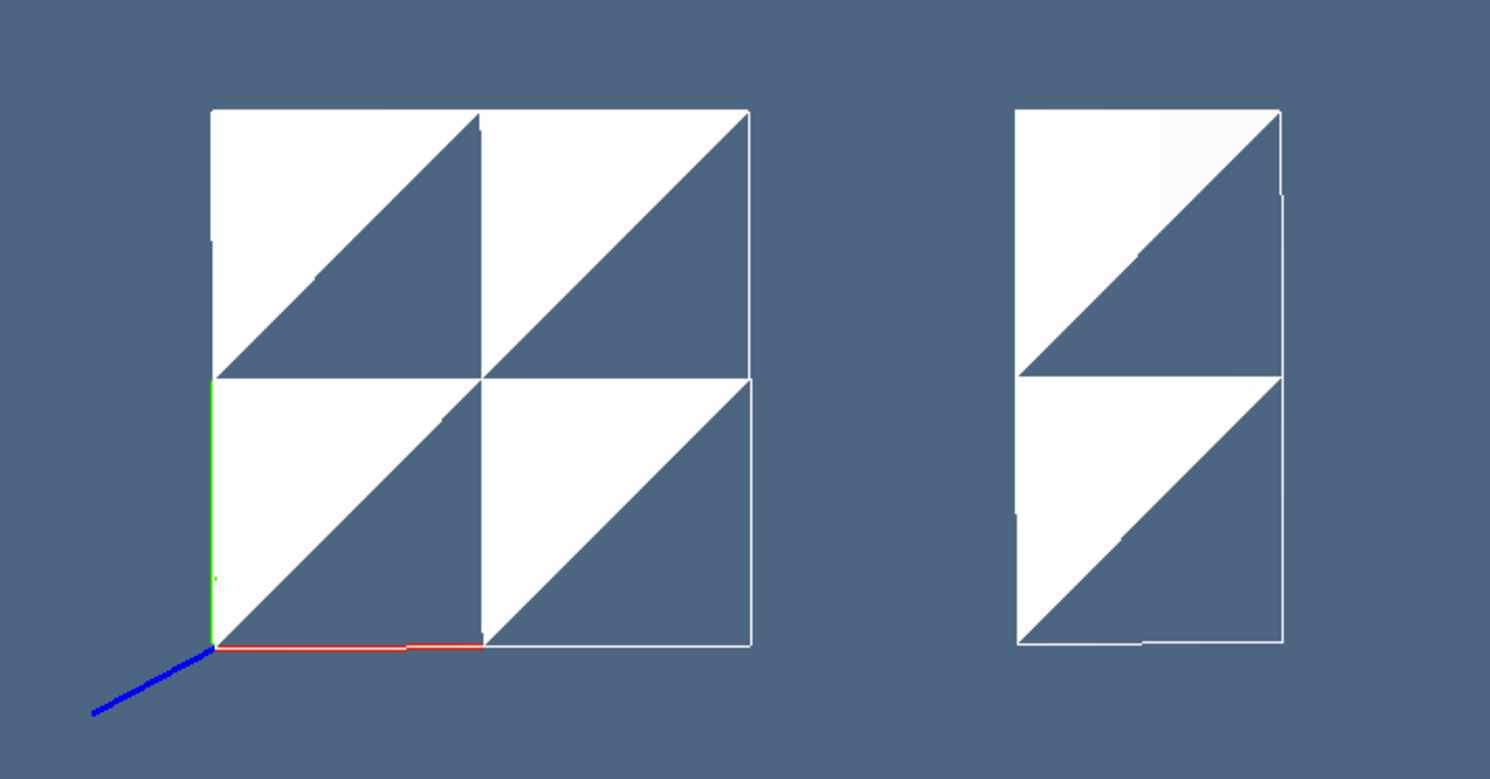
\includegraphics[width=0.405\linewidth]{images/assembly1} 
   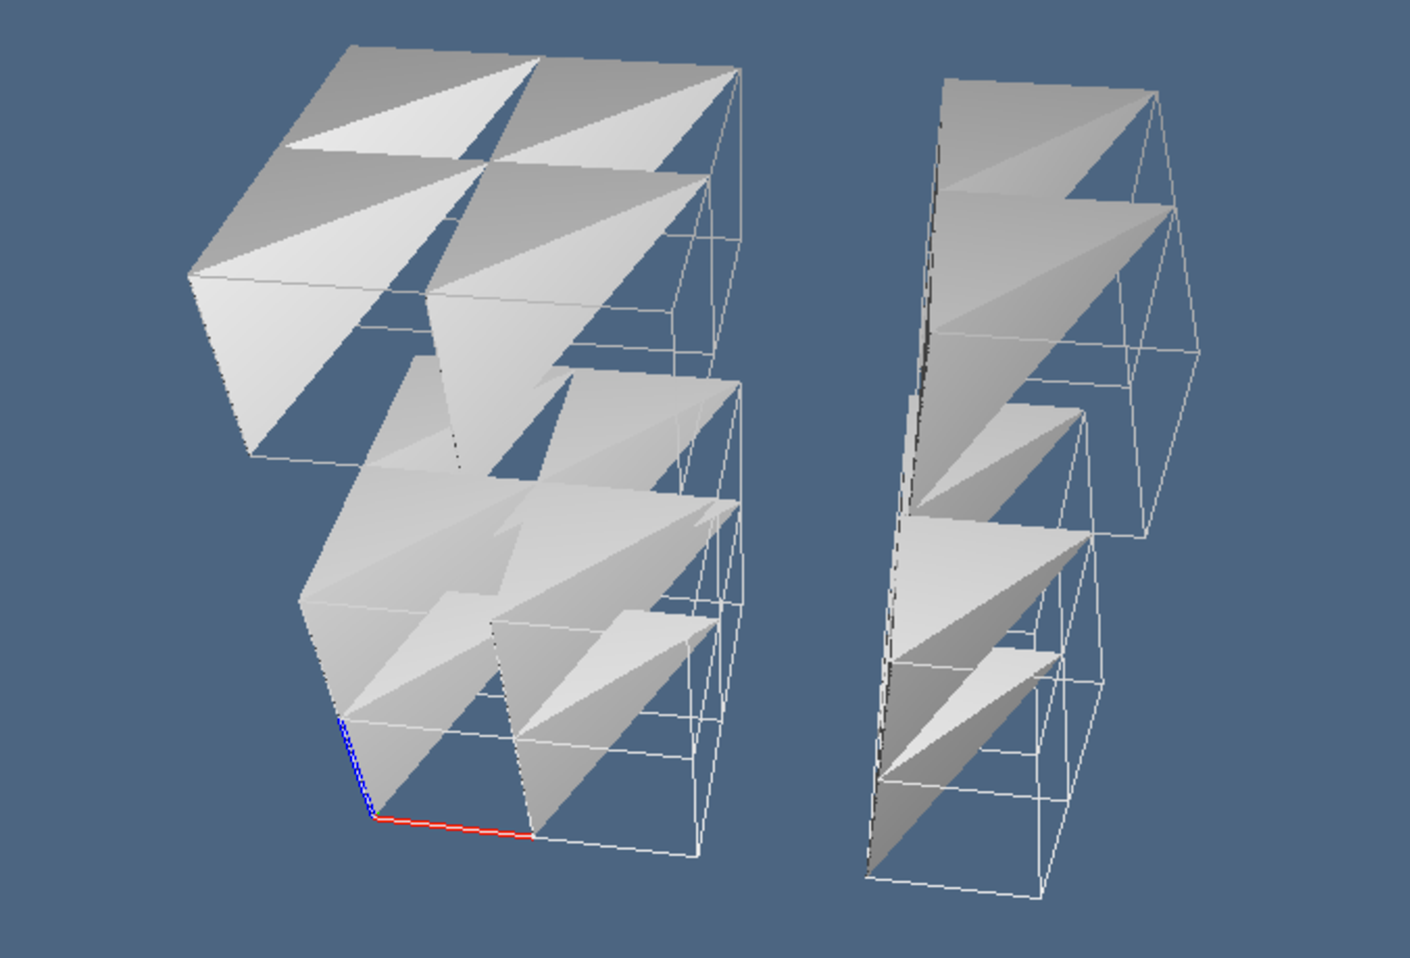
\includegraphics[width=0.315\linewidth]{images/assembly2} 
   \caption{(a) Assemblies of squares and triangles; (b) assembly of cubes and tetrahedra.}
   \label{fig:example}
\end{figure}

%-------------------------------------------------------------------------------
@D Definition of 1-dimensional LAR models 
@{geom_0,topol_0 = [[0.],[1.],[2.],[3.],[4.]],[[0,1],[1,2],[3,4]]
geom_1,topol_1 = [[0.],[1.],[2.]], [[0,1],[1,2]]
mod_0 = (geom_0,topol_0)
mod_1 = (geom_1,topol_1)
@}
%-------------------------------------------------------------------------------

%-------------------------------------------------------------------------------
@D Assembly generation of squares and triangles
@{squares = larModelProduct([mod_0,mod_1])
V,FV = squares
simplices = pivotSimplices(V,FV,d=2)
VIEW(STRUCT([ MKPOL([V,AA(AA(C(SUM)(1)))(simplices),[]]),
			  SKEL_1(STRUCT(MKPOLS((V,FV)))) ]))
@}
%-------------------------------------------------------------------------------

%-------------------------------------------------------------------------------
@D Assembly generation  of cubes and tetrahedra 
@{from largrid import *
cubes = larModelProduct([squares,mod_0])
V,CV = cubes
simplices = pivotSimplices(V,CV,d=3)
VIEW(STRUCT([ MKPOL([V,AA(AA(C(SUM)(1)))(simplices),[]]),
			  SKEL_1(STRUCT(MKPOLS((V,CV)))) ]))
@}
%-------------------------------------------------------------------------------







\bibliographystyle{amsalpha}
\bibliography{larcc}

\end{document}
